\documentclass[12pt]{article}
\usepackage{graphicx}
\usepackage[margin=2cm]{geometry}

\usepackage{amsmath}
\usepackage{amssymb}
\usepackage{amsthm}

\newtheorem{theorem}{Theorem}[section]
\newtheorem{lemma}[theorem]{Lemma}


\title{A Continuous Model Of Behavioural Phenotype: An Example Of
  Interaction Between \textit{Pieris brasicae} And
  \textit{Trichogramma} Wasps}

\author{Kelly Black\thanks{Coresponding Author, kjblack@gmail.con},
  \and Malcolm R Adams, \and Aladeen Al Basheer, \and Caner Kazanci,
  \and Bernard Patten, \and Stuart Whipple, \and Sofya Zaytseva}

\begin{document}

\maketitle

\section{Introduction}

The impact of variation of animal personalities on broad population
dynamics is receiving a great deal of
attention\cite{doi:10.1111/j.1461-0248.2010.01536.x}.  The variation
in animal behaviours as well as the variation in the coresponding
genetic basis for animal personalities plays a role in the broader
population dynamics of the species as well as the other animals that
interact with the species. A variety of mathematical models are being
developed to explore this important aspect of interactions. The models
include compartment models, stochastic, agent based models, as well as
combinations of these approaches. One difficulty, though, with such
approaches is the challenge of developing appropriate analytic tools
to examine the general properties of the resulting models.

We propose an approach that assumes a continuous distribution
associated with one behavioural aspect of an animal's behaviour. In
this initial exploration of a novel approach a relatively
straight-forward interaction is chosen. The example chosen is based on
the interactions between parasitic wasps, \textit{Trichogramma} Wasps,
and the butterfly \textit{Pieris
  brasicae}\cite{10.1093/beheco/arq007}.  The propensity of
\textit{Pieris brasicae} to employ a chemical associated with mating
behaviour is modeled as a continuous distribution, and a distributed
model is developed to approximate the resulting interactions.

In this treatment we approximate the system as consisting of two
species. Finding and parasitizing the butterflies' eggs requires a
relatively long interaction time, and a predator-prey relationship is
assumed. In particular, the predation rates are approximated using a
type II response. Due to the variation in behaviour, though, we adapt
the standard Holling response function for this new situation.

We first provide a more detailed overview of behavioural phenotypes
including some previous efforts to model the phenomena. Next, the
model used to provide insight into the phenomena is developed
including a re-derivation of a type II response assuming a continuous
variation in one behaviour. Following the derivation of the model, the
numerical approximation to the distributed system is briefly
discussed. Finally, some results from our numerical explorations are
provided.

\section{Behavioural Phenotype}
\label{section:behaviouralPhenotype}

The primary motivation for why the distribution of how animals behave
and interact is given in this section. We begin with a discussion of
the basic idea of behavioural phenotype. Next, a brief overview of
existing modeling efforts is provided. Finally a specific example of
social spiders is discussed, and in this example the phenomena is
directly observed and provides context for the importance of the
general phenomena.

A number of authors have noted the importance of the role of variation
in a species' habits or
genetics\cite{doi:10.1111/j.1461-0248.2010.01536.x,doi:10.1086/687235,mierzejewski_horn_luong_2019,SANTICCHIA20191}. We
begin this discussion with the survey provided by Kortet, \textit{et
  al}\cite{doi:10.1111/j.1461-0248.2010.01536.x}. The authors note
that within any large group of animals certain behaviours can vary
across the population. They go on to propose that the diversity of
behaviours can profoundly impact the broader dynamics of the
population of the animals as well as animals with a shared
interdependence.

Kortet, \textit{et al}\cite{doi:10.1111/j.1461-0248.2010.01536.x} note
the impact of variation in the distribution of behaviour. They note
some potential challenges this recognition implies, as well. One
challenge is the difficulty to identify and quantifyi the distribution
of animal personalities in a given population. A specific example
relates to the capture of Pumpkin Seed
Fish\cite{doi:10.1037/0735-7036.107.3.250}, and the methods used to
capture individuals in a population can result in a biased estimate.
Some methods may be more or less likely to capture a subset of
individuals based on the individuals' behaviours.

% https://www.semanticscholar.org/paper/Fish-behavioral-types-and-their-ecological-Mittelbach-Ballew/a381cb0b64a8107c694454e940fd7972263a8b77
% https://www.semanticscholar.org/paper/Are-most-samples-of-animals-systematically-biased-Biro/72eaa11f60d3b211f34ab04ff95211307978223b

A wide array of approaches to model the phenomena have been
explored. The different approaches include stochastic
models\cite{Keeling65}, agent based models\cite{doi:10.1086/687235},
hybrid models employing compartment models based on a stochastic
distribution\cite{doi:10.1098/rspb.2001.1599},a and statistical
models\cite{SuperspreadingLloyd}. A brief description of some of these
approaches is provided below.

An example of a stochastic is provided by Keeling and
Grenfel\cite{Keeling65}. They note that the dynamics of the incidence
of measles is influenced by how the incubation time varies across
individuals. In response to this observation they modified standard
disease modeling by adding a convolution of a time delay.


Another adaptation for a similar problem was proposed by
Lloyd\cite{doi:10.1098/rspb.2001.1599}. In this case the rates that
infected individuals leave the infected class is based on stochastic
distribution. The phenomena was modeled by making use of a large
number of compartments, and entry into the different classes is
governed by the underlying probability distribution.

An example of a statistical approach that highlights the importance of
the phenomena is given by Lloyd-Smith \textit{et
  al}\cite{SuperspreadingLloyd}. In their work the transmission of
disease is examined using a branching process. The varying
transmission rates between individuals is treated as a given
probability distribution, and the variation in the differences can
result in large differences in the estimation of transmission rates.

A mathematical model examining the interactions within a colony of
social spiders, \textit{Stegodyphus dumicola}, is provided by
Pinter-Wollman, \textit{et al}\cite{doi:10.1086/687235}. The focus of
their work is in examining the impact of different boldness levels of
a key individual.  They note that a small number of individuals within
a colony may exhibit different levels of aggression, and a small
number of individuals can have a disproportionate impact in the
broader success of the colony.

As a means to model this important aspect of a colony, Pinter-Wollman,
\textit{et al}\cite{doi:10.1086/687235} provide a computational model
consisting of an agent based model with a stochastically generated
population. Their approach is based on a small number of rules that
result in a distribution of behaviours. The temporal interactions
within the colony are approximated via discrete time steps and
stochastic decision making. The external interactions are approximated
using an ordinary differential equation model.

In the resulting statistical analyses, Pinter-Wollman, \textit{et
  al}\cite{doi:10.1086/687235} found that different levels of boldness
within key individuals resulted in a difference in the mean boldness
levels of a broader group. For example, they found the differences in
boldness impacted the rate of capture of prey. They also found that
the rules themselves also impacted the disease dynamics within the
population.


\section{Modeling Genetic Variance As a Continuous Distribution}

Rather than construct a compartmental model or an agent based model, a
continuous, distributed parameter model is proposed. The resulting
model for the example system is a coupled partial differential
equation and an ordinary differential equation. Prior to the
derivation itself an overview of the specific system, the interactions
between butterflies and a parasitic wasp, are discussed. Next the
model is derived. Finally, and analysis of a simplified system of
ordinary differential equations is examined as a way to gain some
preliminary insights into the resulting system.

\subsection{Butterflies v. Wasps}
\label{butterflyVWasps}

The example of social spiders was briefly discussed earlier, but the
model developed here focuses on the interaction between butterflies,
\textit{Pieris brasicae}, and \textit{Trichogramma} wasps that prey on
the butterflies' eggs. The interactions between these populations has
received a good deal of attention
\cite{PMC2797620,doi:10.1111/j.1439-0418.1986.tb00834.x,Figueroa2010AttractionOT,10.3389/fpls.2019.01768}. We
focus on the results of one source in particular Huigens \textit{et
  al}\cite{10.1093/beheco/arq007}. In their work, the authors state
that the pressure placed on the butterfly population due to the wasps'
interactions results in a change in the long term behaviour of the
butterfly population.

The source of this pressure is the nature of the mating practices of
\textit{Pieris brasicae}. In order to attract a mate, the female
butterflies tend to emit a pheromone designed to attract the males to
the females. After copulation, though, it is not in either the
female's nor the male's best interest to continue to attract other
butterflies. In response, the male butterflies have a propensity to
apply another pheromone, referred to as an anti-aphrodisiac, that will
reduce the effectiveness of the original pheromone emitted by the
female.

The downside to the use of the pheremone is that it exposes the eggs
to a greater risk of predation. Some species of \textit{Trichogramma}
wasps parasitize the eggs of the butterflies. Sometimes they
physically attach themselves to a butterfly and ride it until the
butterfly begins to attach their eggs in a preferable location. The
wasps are able to detect the presence of the anti-aphrodisiac which is
correlated with an increased probability that a butterfly with the
anti-aphrodisiac is more likely to lay eggs. In response, the wasps
are more likely to ride on a butterfly if it detects the
anti-aphrodisiac. It is important to note this method of predation on
a butterfly's eggs requires a non-trivial time commitment with respect
to handling and detecting the presence of the eggs.

The authors\cite{10.1093/beheco/arq007} note that the probability that
a male will make use of the anti-aphrodisiac varies between
individuals. There are different trade-offs in the use of the
anti-aphrodisiac, but the authors found that the wasps' actions are
applying direct evolutionary pressure with respect to the habits of
the butterflies. In particular they provide evidence that the
distribution of the propensity of the male butterflies to make use of
the anti-aphrodisiac is changing in time, and over time a growing
number of butterflies are less likely to engage in the behaviour.

\subsection{Modeling Behavioural Phenotype As a Continuous
  Distribution}

As mentioned in section \ref{section:behaviouralPhenotype}, a number
of options have been employed to model a distribution of behavioural
preferences in a given population. These methods include compartmental
models, agent based models, and hybrids of these two models. One
potential issue, though, is that the number of variations can be quite
high. For example Abolins-Abols \textit{et al} examined a system in
which over 120 genetic sites determine a given animal's
propensity\cite{doi:10.1111/mec.14878}. The resulting number of
combinations of such sites can be extremely high.

Rather than treat the possible behaviours as a discrete distribution
we instead treat it as a continuous distribution. The way in which
this manifests itself within a model is to treat the population as a
distribution with respect to the new parameter. This new independent
variable is introduced within the model, and the parameter is now a
function that will vary as the independent variable varies.

At first glance, this is akin to a Bayesian statistical approach that
is often used to estimate the value of a
parameter\cite{doi:10.1111/j.1467-9868.2007.00610.x,Fitzpatrick_1991}. In
these approaches a probability distribution is assumed to describe the
likelihood that a parameter takes on a given range of values. In our
case, though, we turn this around and assume that the population
itself varies, and the relative population density depends on the
underlying variable.

A question arises about how to translate the impact of this parameter
within a given model. In this initial examination of the approach we
employ the simplest option and assume a linear impact with respect to
the new independent variable. In particular, for the interactions
between the butterflies and wasps we track the population densities of
the two populations. Due to the time scale of interactions between the
butterflies and wasps as well as direct mortality of the interaction
we assume a predator-prey relationship rather than a disease like
relationship modeled in other parasitic systems.

The system is adapted from Tewa, \textit{et al}\cite{TEWA20134825}. We
first focus on the model as a system of ordinary differential
equations and later adapt it for the distributed system described
above. The basic assumption is that in the absence of predation the
butterfly population will act in a way consistent with the logistic
equation. In the absence of any butterflies the wasps will slowly die
out. For this particular system, however, \textit{brasicae} is a
generalist predator, and this is an assumption that should be
revisited beyond this initial investigation. Finally, the predation by
\textit{brasicae} requires substantial time for the wasp to follow the
moths and oviposit its eggs, and the rate of predation can be
approximated as a type II response\cite{TEWA20134825}.  The resulting
ordinary differential equation is given by
\begin{eqnarray}
  \label{eq:initialSystem1}
  \frac{d}{dt} b(t) & = & \alpha \cdot b(t) (K - b(t)) - \gamma \cdot w(t) \frac{b(t)}{c+b(t)}, \\
  \label{eq:initialSystem2}
  \frac{d}{dt} w(t) & = & -d \cdot w(t) + g \cdot w(t) \frac{b(t)}{c+b(t)}.
\end{eqnarray}
The density of butterflies is modeled by the function $b(t)$, the
density of wasps is modeled by the function $w(t)$, and the parameters
$\alpha$, $\gamma$, $d$, and $g$ are positive constants. 

For this situation, though, there is a distribution associated with
the butterflies' propensity to make use of the anti-pheromone. We do
not model the male and female populations separately, but treat them
as a single population that intermingles in a relatively uniform
fashion. The propensity for a butterfly to make use of the
anti-pheromone depends on a new parameter, $\theta$. The value of
$\theta$ is assume to vary between $0$ and some positive constant,
$L$, and the larger the value of $\theta$ the more likely an
individual is to make use of the anti-pheromone. The distribution of
the population of butterflies is now dependent on both the time and
the new parameter,
\begin{eqnarray}
  b & = & b(t,\theta).
\end{eqnarray}

Our first task is to determine how the type II, or Holling type
response, should be expressed in this new context. Formal derivations
of the response function for the case given in equations
(\ref{eq:initialSystem1}) and (\ref{eq:initialSystem2}) are provided
bye Dawes and Sousa\cite{DAWES201311}.  In the derivation here,
however, we follow the approach in Holling's original
discussion\cite{holling_1959A,holling_1959B}. We begin by finding an
expression that relates the number of eggs parasitized by a single
wasp, $Y(\theta)$, which is assumed to be a linear relationship,
\begin{eqnarray}
  \label{eq:processingTime}
  Y(\theta) & = & r T_{\mathrm{search}}(\theta) b(t,\theta) p(\theta),
\end{eqnarray}
where $T_{\mathrm{search}}$ is the search time required by the wasp to
find the location of a butterfly's clutch. The motivation for this is
that the higher the value of $\theta$ the higher the success rate for
a given wasp.  The time a wasp requires to parasitize the clutch is
assumed to be proportional to the number of eggs, and the total time
is
\begin{eqnarray}
  \label{eq:totalEgglayingTime}
  T_{\mathrm{total}}(\theta) & = & T_{\mathrm{search}}(\theta) + \beta Y(\theta).
\end{eqnarray}
Substituting the search time found in equation
(\ref{eq:totalEgglayingTime}) back into equation
(\ref{eq:processingTime}) results in an expression for the rate of
predation per wasp,
\begin{eqnarray}
  \label{eq:waspPredationRate}
  Y(\theta) & = & \frac{r T_{\mathrm{total}} b(t,\theta) p(\theta)}{1 + \beta r b(t,\theta) p(\theta)}.
\end{eqnarray}

In this case $p(\theta)$ represents the impact associated with the use
of the anti-pheromone. As $\theta$ increases the more likely an
individual butterfly is to make use of the anti-pheromone and the more
likely a wasp is to locate and ride along with a butterfly. The
function, $p(\theta)$, will be used to balance the positive and
negative impacts in the growth as well as the predation terms in
equation (\ref{eq:initialSystem1}), and the parameters $\alpha$ and
$\gamma$ provide relative scales for the two impacts. Note that we can
normalize $p(\theta)$ because it is scaled by the parameter $r$.


Turning back to equation (\ref{eq:waspPredationRate}), the rate of
predation can now be approximated.  The result can be immediately
substituted into equation (\ref{eq:initialSystem1}) in the more
traditional form as
\begin{eqnarray}
  \label{eq:butterflyPredationRate}
  \gamma \cdot w(t) \frac{p(\theta) b(t,\theta) }{c +  p(\theta) b(t,\theta)}
\end{eqnarray}
The values of the constants $c$ and $\gamma$ are the result of
combining the terms that include $r$, $\beta$, and $T_\mathrm{total}$
in equation (\ref{eq:waspPredationRate}).  Equation
(\ref{eq:initialSystem2}), though, is the rate of predation for the
single wasp population, so the impact for the wasps must be
accumulated across the entire butterfly population,
\begin{eqnarray}
  \label{eq:totalWaspPredationRate}
  \int^L_{\theta=0} g \cdot w(t) \frac{p(\theta) b(t,\theta) }{c + p(\theta) b(t,\theta)} ~ d\theta.
\end{eqnarray}

We are almost ready to put these terms together for the current
model. It is assumed that the mixing and interactions within the
butterfly population is uniform, and the diffusion of the trait
roughly follows Fick's law\cite{logan2006applied}. Here, a second
order derivative term approximates the sharing of the genetic
information relative to the propensity to use the
anti-aphrodisiac. The result is a coupled PDE and ODE system given by
\begin{eqnarray}
  \label{eq:odePDE1}
  \frac{\partial}{\partial t} b(t,\theta) & = &
      \alpha \cdot p(\theta) b(t,\theta) (K - b(t,\theta))
      - \gamma \cdot w(t) \frac{p(\theta) b(t,\theta)}{c+p(\theta)b(t,\theta)}
      + \mu \frac{\partial^2}{\partial \theta^2} b(t,\theta) , \\
  \label{eq:odePDE2}
  \frac{d}{dt} w(t) & = & -d \cdot w(t) +
      \int^L_{\theta=0} g \cdot w(t) \frac{p(\theta) b(t,\theta) }{c + p(\theta) b(t,\theta)} ~ d\theta.
\end{eqnarray}

As previously noted, the function $p(\theta)$ is assumed to be an
increasing function for $0\leq\theta\leq L$, and $p(0)>0$. If it is
zero then equation (\ref{eq:initialSystem1}) will indicate no growth
and no predation. We can assume $p(0)$ is a minimal value, $p(0)=a$,
and the relationship has a positive slope. We examine the simplest
such relationship, a linear function.

This function is scaled separately in equations (\ref{eq:odePDE1}) and
(\ref{eq:odePDE2}), and the function can be scaled in an arbitrary
manner. We choose to scale the function so that its integral is one,
and the resulting normalized form is
\begin{eqnarray}
  \label{eq:linearFormP}
  p(\theta) & = & a + \frac{2(1-aL)}{L^2} \theta.
\end{eqnarray}
One immediate restriction on the parameters requires that
$0<aL<1$. The interpretation of the slope is that the greater the
value of the slope then the greater the variation is in the observed
trait.

The variables can be scaled as $b\rightarrow \bar{B}\hat{b}$,
$w\rightarrow \bar{W}\hat{w}$, $t\rightarrow \bar{T}\hat{t}$, and
$\theta\rightarrow \bar{\Theta}\hat{\theta}$. We choose $\bar{B}=K$,
$\bar{W}=\frac{\alpha K^2 a}{\gamma}$, $\bar{T}=\frac{1}{\alpha K a}$,
and $\bar{\Theta}=L$. The resulting system can be reduced to the
following form
\begin{eqnarray}
  \label{eq:scaledodePDE1}
  \frac{\partial}{\partial t} b & = &
      \hat{p}(\theta) b (1 - b)
      -  w \frac{\hat{p}(\theta) b}{c+\hat{p}(\theta)b}
      + \mu \frac{\partial^2}{\partial \theta^2} b , \\
  \label{eq:scaledodePDE2}
  \frac{d}{dt} w & = & -d \cdot w +
      \int^1_{\theta=0} g \cdot w \frac{\hat{p}(\theta) b }{c + \hat{p}(\theta) b} ~ d\theta,
\end{eqnarray}
where
\begin{eqnarray}
  \hat{p}(\theta) & = & 1 + m \cdot \theta.
\end{eqnarray}
The domain for the scaled independent variable, $\theta$, is
$0\leq\theta\leq 1$. As previously noted, the slope, $m$, can be
interpreted to indicate how much variation in the trait is present in
a population. The larger $m$ is the greater the amount of variation.
With respect to the PDE, Neumann boundary conditions are used in the
subsequent numerical approximations below. A variety of initial
conditions have been explored, and they are described in the results
section, section \ref{section:results}.


\subsection{Parameter Dependence on Stability of the System}
\label{subsection:parameters}

Prior to examining the behaviour of the distributed system given in
equations \ref{eq:odePDE1} and \ref{eq:odePDE2}, the potential
restrictions on the parameters are explored. We first examine a
simplified system based on a system of ordinary differential
equations.  The focus is on the impact of the parameters of the
system, and a more complete analysis is provided in Appendices
\ref{appendix:otherFixedPoints} and \ref{appendix:stability}.

The simplified system is found by examining an ODE with a similar form
as the distributed system. By assuming that the distribution of the
butterflies is a constant consistent with a single value of $\theta$,
the system is approximated by the following system of ODEs:
\begin{eqnarray}
  \label{eq:scaledODE1}
  \frac{d}{dt} b(t) & = &
      \hat{p}(\theta) b(t) (1 - b(t))
      -  w(t) \frac{\hat{p}(\theta) b(t)}{c+\hat{p}(\theta)b(t)}, \\
  \label{eq:scaledODE2}
  \frac{d}{dt} w(t) & = & -d \cdot w(t) +
       g \cdot w(t) \frac{\hat{p}(\theta) b(t) }{c + \hat{p}(\theta) b(t)}.
\end{eqnarray}

By focusing on the system of ODEs, we can examine an approximation to
the system by treating the variable $\theta$ as a fixed parameter and
can gain some insight into the distributed system. The analysis in
this section focuses on the stability of the linearized system at the
nontrivial fixed point. More details about the other fixed points is
provided in Appendix \ref{appendix:otherFixedPoints}

We first determine the nullclines for the system.
The $b$-nullclines for the system in the $b-w$ plane are given by
\begin{eqnarray}
  \label{eq:bnullclines}
  b & = & 0, \\
  w & = & (1-b)(c+b\cdot \hat{p}(\theta)).
\end{eqnarray}
The second $b$-nullcline is a parabola opening downward, and the vertex is located at
$b=\frac{\hat{p}(\theta)-c}{2\hat{p}(\theta)}$. The $w$-nullclines are given by
\begin{eqnarray}
  \label{eq:wnullclines}
  w & = & 0, \\
  b & = & \frac{cd}{(g-d)\hat{p}(\theta)}.
\end{eqnarray}
The second $w$-nullcline is a vertical line in the $b-w$ plane. In
order for a fixed point to exist in the first quadrant an immediate
restriction on the parameters requires that $g>d$.  Given the
nullclines, the only fixed point that occurs in the first quadrant
away from an axis is at $b=\frac{cd}{\hat{p}(\theta)(g-d)}$ and
$w=\left(\frac{cd}{g-d}+c\right)
\left(1-\frac{cd}{\hat{p}(\theta)(g-d)}\right)$.

The Jacobian for the system in equations (\ref{eq:scaledODE1}) and
(\ref{eq:scaledODE2}) at the fixed point is
\begin{eqnarray}
  J & = &
          \left[
          \begin{array}{rr}
            J_{11} & J_{12} \\
            J_{21} & 0
          \end{array}
          \right],
\end{eqnarray}
where
\begin{eqnarray}
  \label{eq:jacobian}
  J_{11} & = & \hat{p}(\theta)(1-2b) - w \hat{p}(\theta)\frac{c}{(c+\hat{p}(\theta)b)^2}, \\
  J_{12} & = & \frac{-b\cdot \hat{p}(\theta)}{c+\hat{p}(\theta)b}, \\
  J_{21} & = & \frac{g\cdot c \cdot w \cdot \hat{p}(\theta)}{(c+\hat{p}(\theta)b)^2}.
\end{eqnarray}
The eigen values of the Jacobian have negative real part when the
trace is negative,
\begin{eqnarray}
  \hat{p}(\theta)(1-2b) - w \hat{p}(\theta)\frac{c}{(c+\hat{p}(\theta)b)^2} & < & 0.
\end{eqnarray}
Substituting the values of $b$ and $w$ for the non-trivial fixed point
yields
\begin{eqnarray}
  \label{eqn:traceNegative}
  \frac{\hat{p}(\theta)-c}{2\hat{p}(\theta)} & < & \frac{cd}{(g-d)\hat{p}(\theta)}.
\end{eqnarray}
This expression can be viewed through another substitution. Let
$u=\frac{cd}{g-d}=\frac{c}{\frac{g}{d}-1}$, and since
$\hat{p}(\theta)>0$ the relationship in equation
(\ref{eqn:traceNegative}) is now
\begin{eqnarray}
  \label{eq:stabilityParameters}
  u & > & \frac{p-c}{2}.
\end{eqnarray}
Note also that under this transformation, the value of the butterfly
density at the fixed point is $\frac{u}{p}$. The scaling in the
original model is based on the carrying capacity which presumes that
\begin{eqnarray}
  \frac{u}{p} & < & 1,
\end{eqnarray}
or 
\begin{eqnarray}
  \label{eq:boundFixedPoint}
  u & < & p.
\end{eqnarray}

A feasible region that implies stability of the fixed point can be
determined in the $u-p$ plane. If the parameters result in a point in
the region bounded by equation (\ref{eq:stabilityParameters}),
equation (\ref{eq:boundFixedPoint}), and $v>0$ then the resulting
fixed point will be linearly stable. A graphical depiction of the
stability region in the $u-p$ plane is shown in Figure
\ref{fig:uvStabilityRegion}.

\begin{figure}[htb]
  \centering
  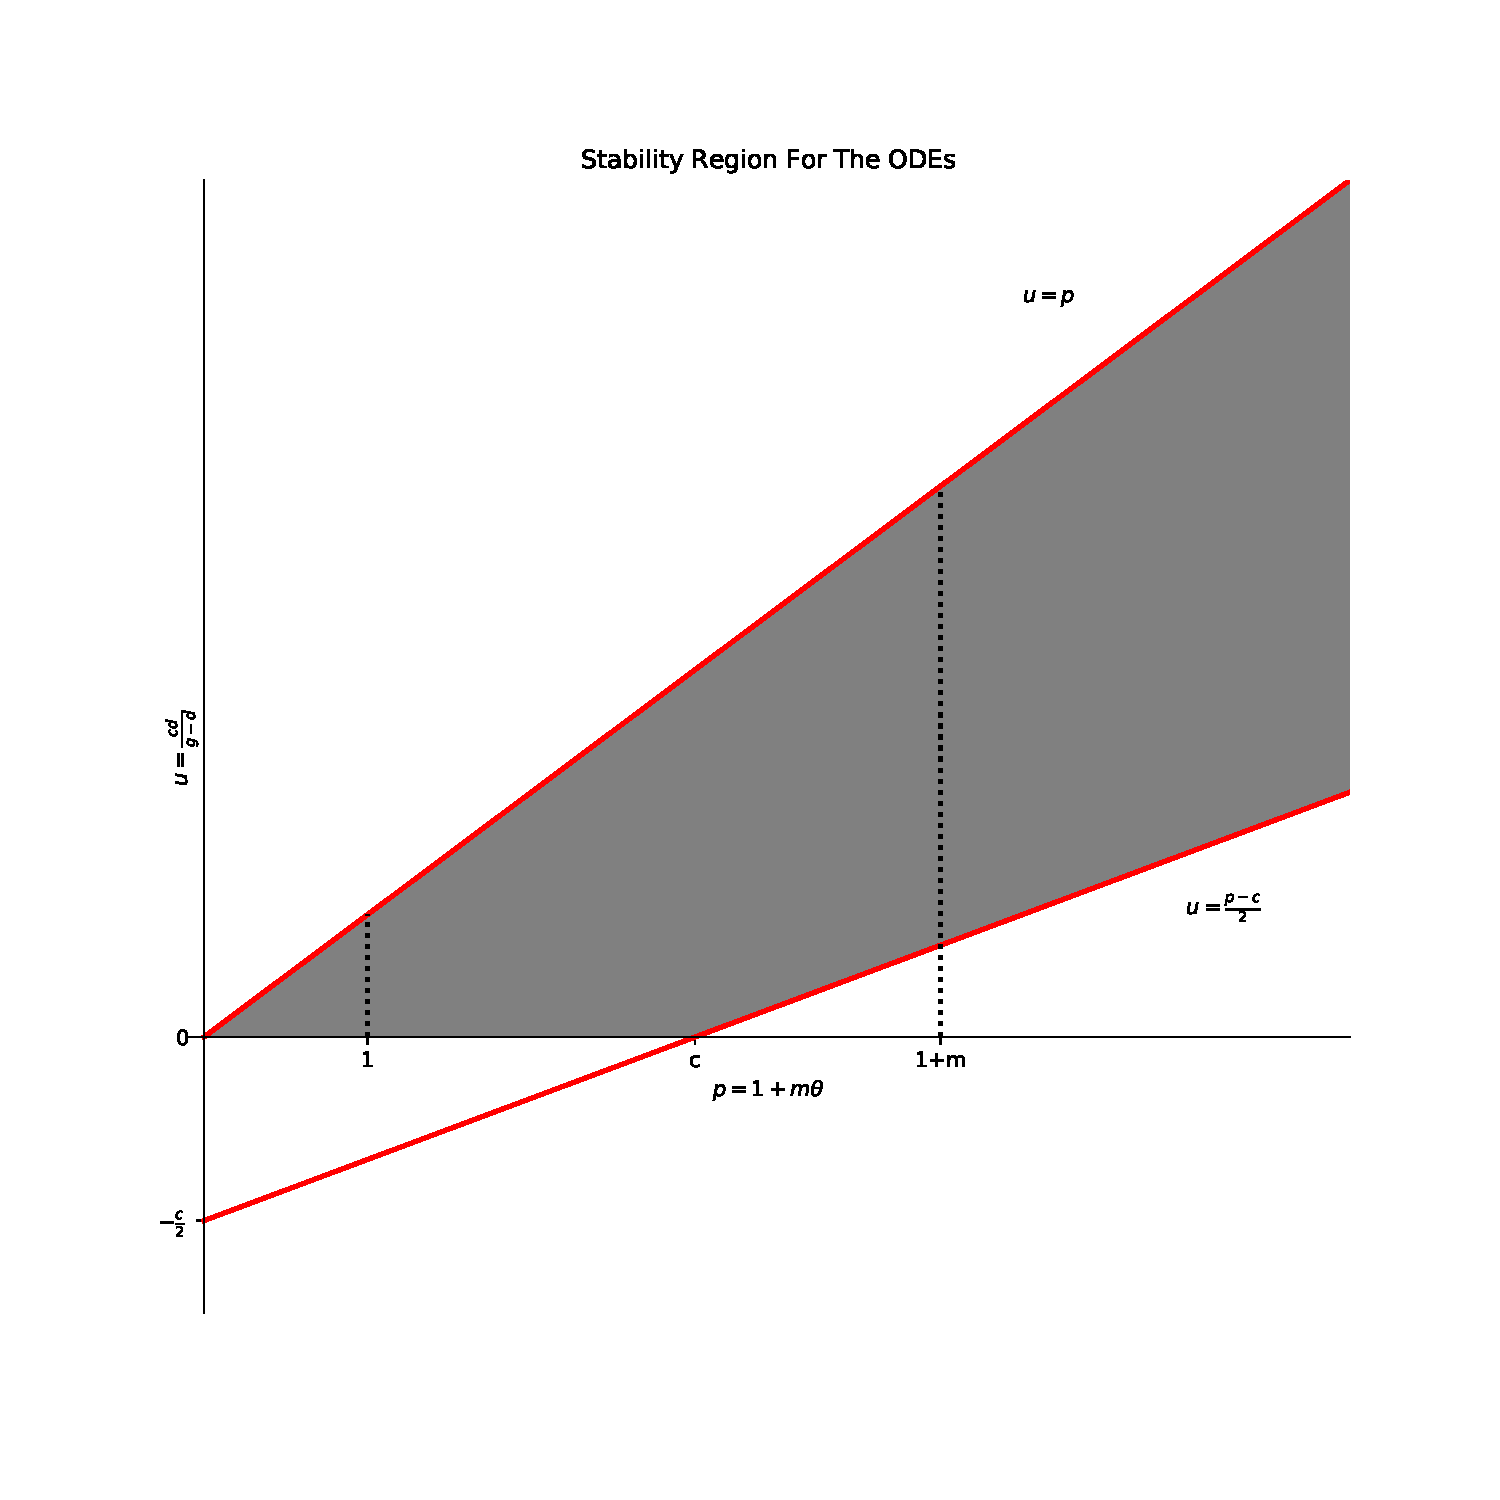
\includegraphics[width=10cm]{img/odeStability-uv-plane.pdf}
  \caption[Stability region in the $u-p$ plane.]{Graphical view of the
    combined feasible and stability region in the $u-p$ plane.}
  \label{fig:uvStabilityRegion}
\end{figure}

In the context of the full, distributed system in equation
(\ref{eq:scaledodePDE1}) and equation (\ref{eq:scaledodePDE2}) the
domain of $\theta$ is $0\leq\theta\leq 1$. For a given set of
parameters the value of $u$ is fully determined. The values of $p$
vary from $p=1$ to $p=1+m$.  The corresponding region in the $u-p$
plane is along a horizontal line segment from $(1,u)$ to
$(1+m,u)$ as shown in Figure \ref{fig:distributedLineSegment}.

\begin{figure}[htb]
  \centering
  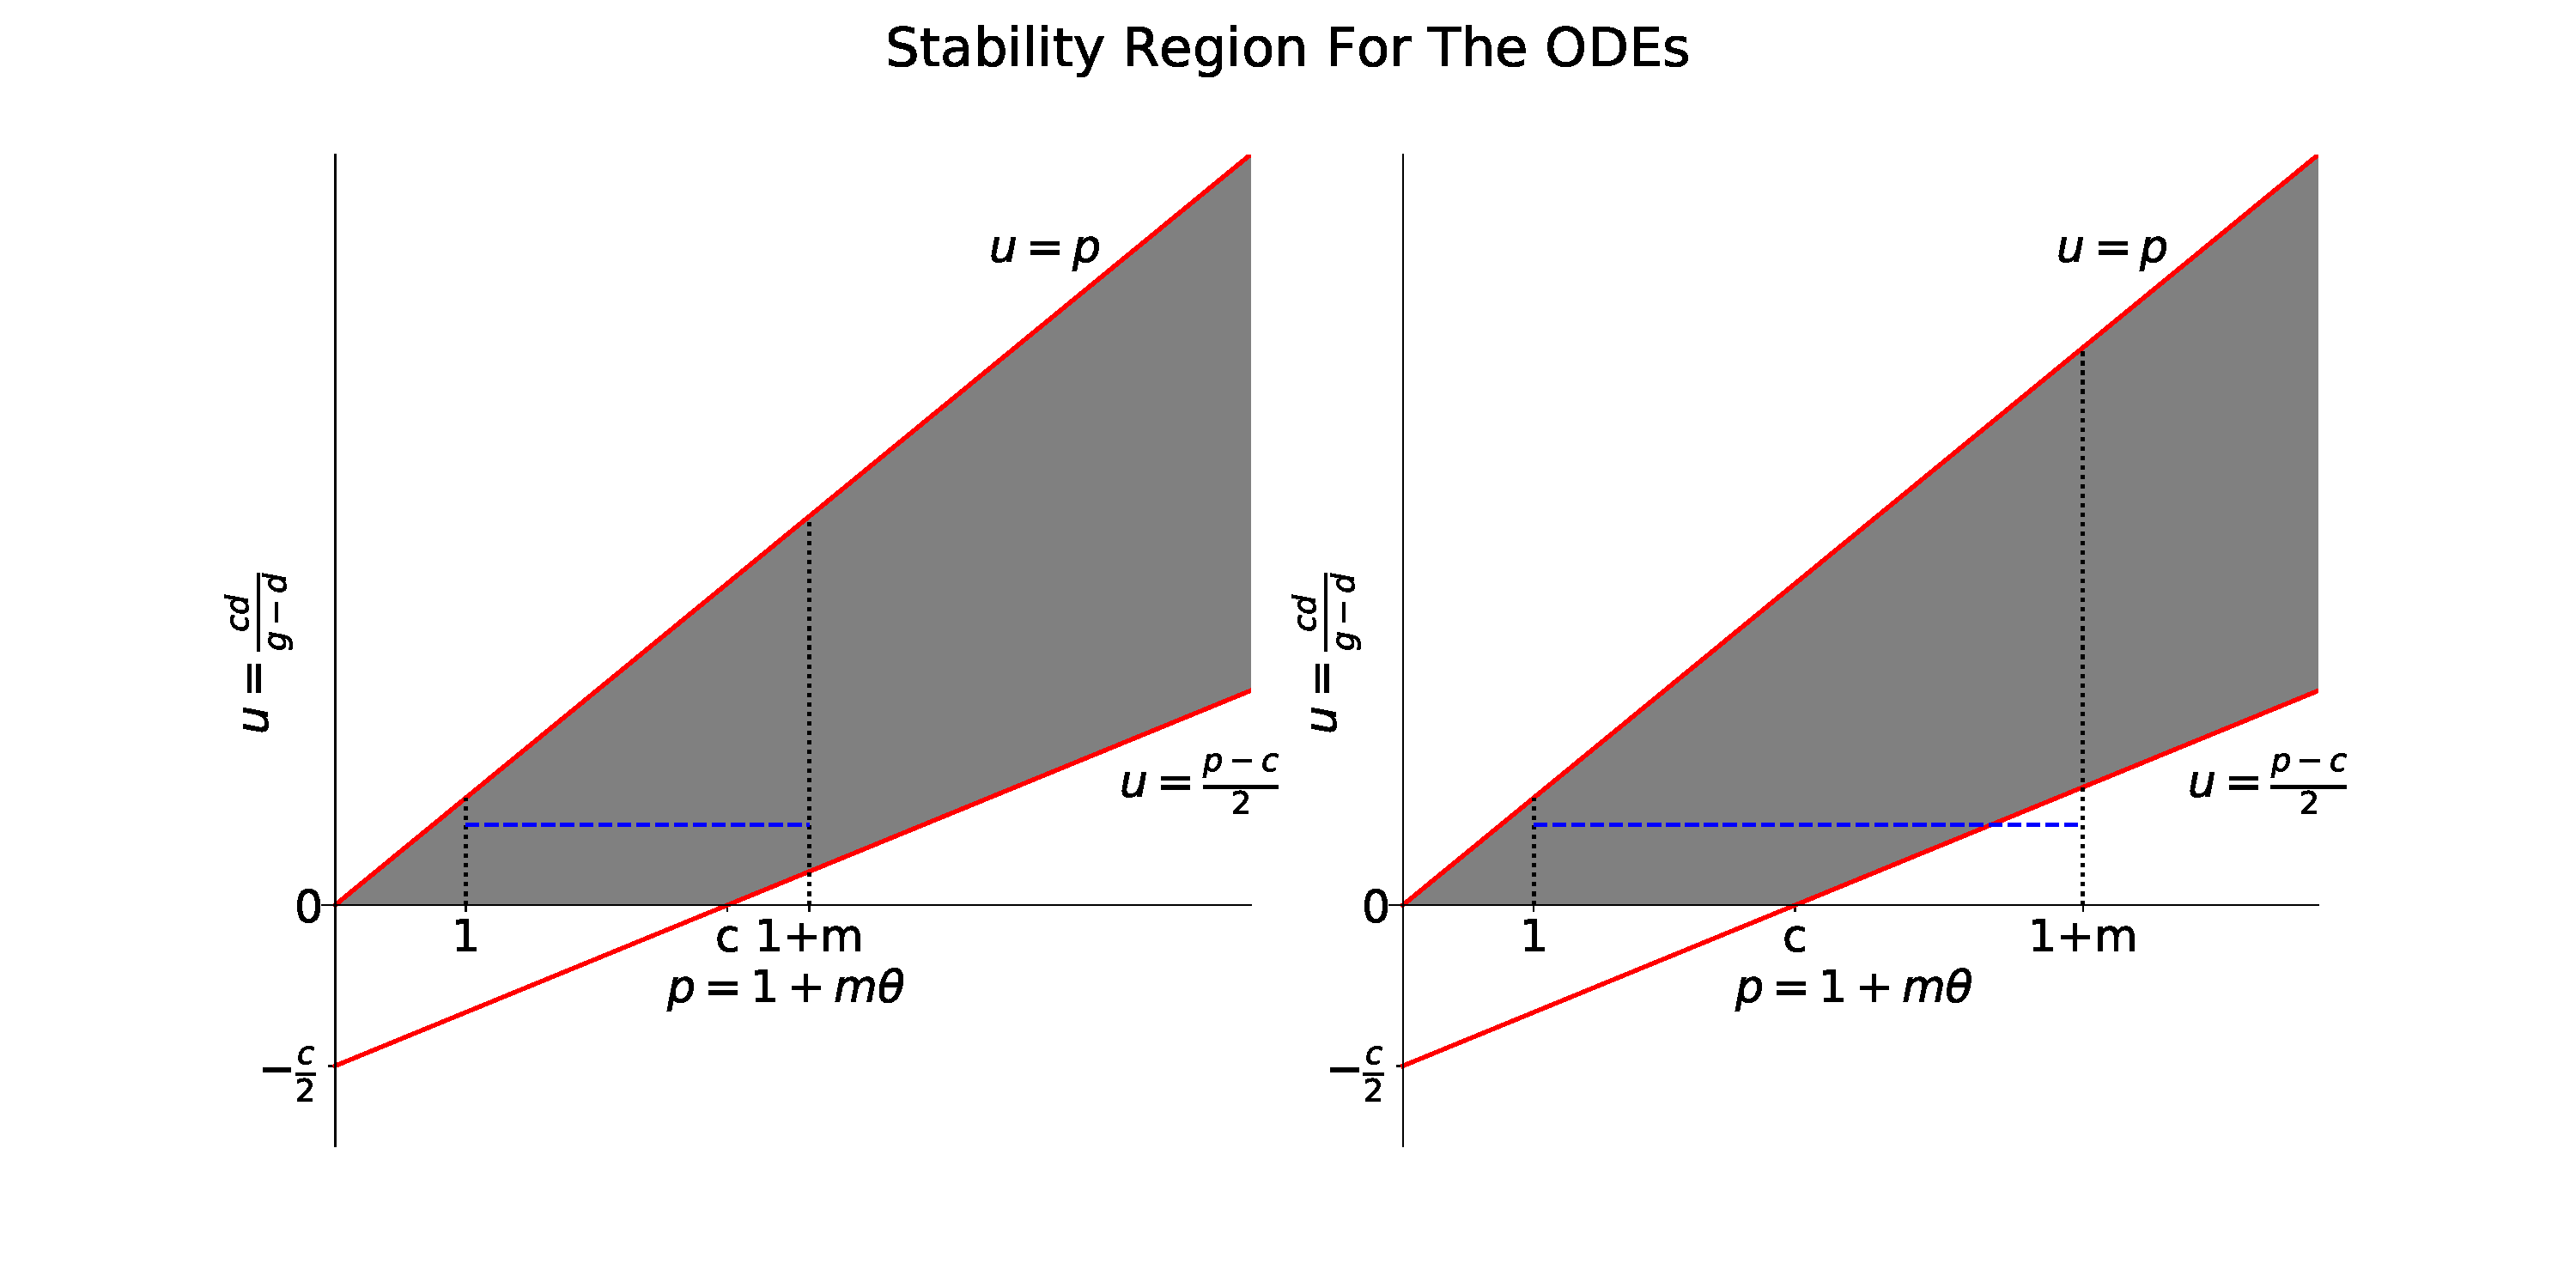
\includegraphics[width=12cm]{img/odeStability-uv-plane-Line.pdf}
  \caption[Domain of the distributed system in the $u-p$
  plane.]{Domain of the parameters for the distributed system for a
    given set of parameters for $0\leq\theta\leq 1$. The dotted line
    represents the values of $\hat{p}(\theta)=1+m\theta$ for all
    values of $\theta$. The figure on the left is an example of a
    smaller value of $m$ while the figure on the right is an example
    of a larger value of $m$. The whole population shown in the figure
    on the left lie in a stable region, while part of the population
    shown in the figure on the right lie in an unstable region.}
  \label{fig:distributedLineSegment}
\end{figure}

\begin{figure}[htb]
  \centering
  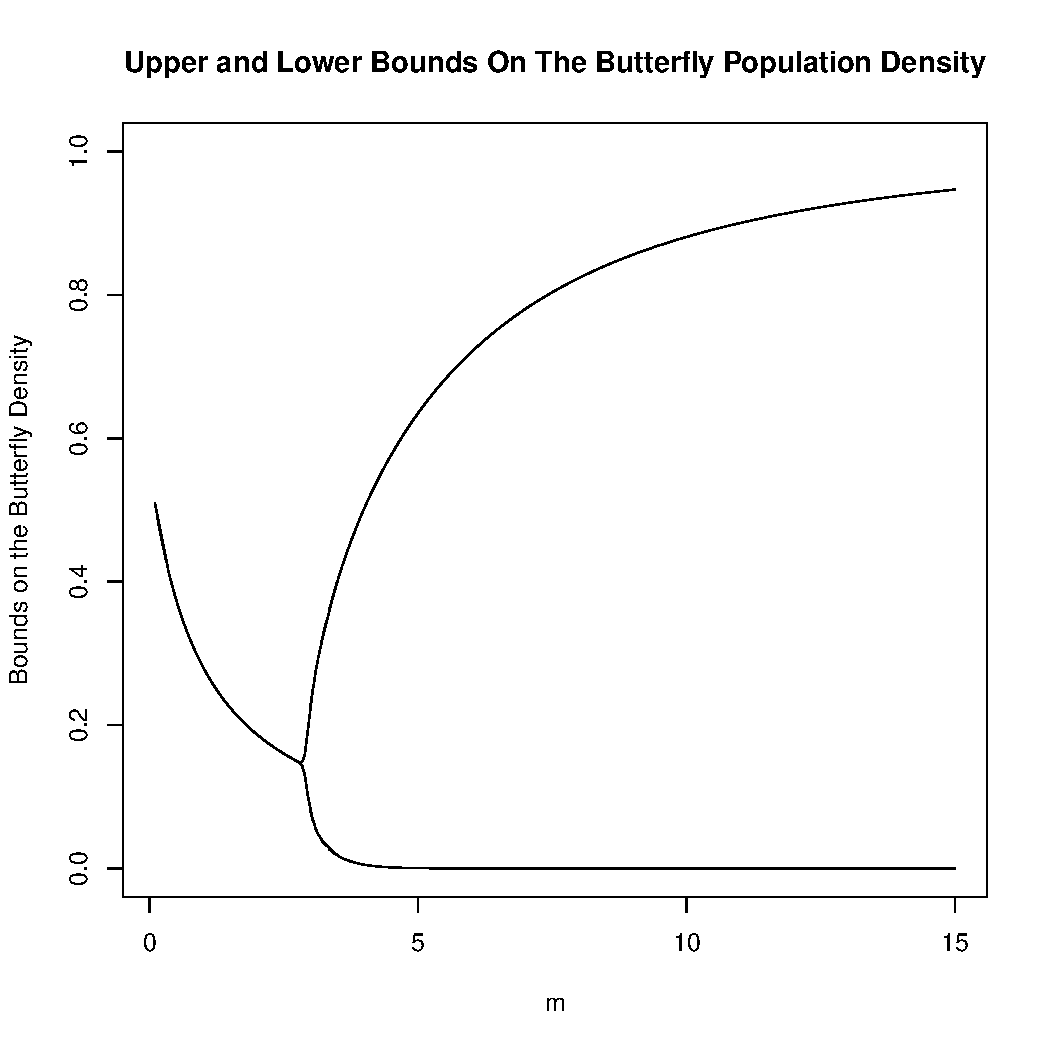
\includegraphics[width=12cm]{img/ODEButterflyBounds.pdf}
  \caption[Upper and lower bounds of the butterfly density.]{The upper
    and lower bounds of the long term density of the butterfly
    population. The population was approximated for different values
    of $m$. The approximation was stopped if it either became close to
    a steady state or a limit cycle.}
  \label{fig:odeButterflyBifurcation}
\end{figure}




\section{Results}
\label{section:results}

A collection of specific approximations is provided. We start with an
examination of the behaviour of the system of ODEs given in equations
(\ref{eq:scaledODE1}) and (\ref{eq:scaledODE2}). Next approximations
of the coupled PDE and ODE from equations (\ref{eq:scaledodePDE1}) and
(\ref{eq:scaledodePDE2}) are provided. In both sets of examples a
numerical exploration of the existance of a stable steady state or
limit cycles is given.

The results given here rely on the numerical approximation of the two
systems previously discussed. In particular approximation for the
system of ODEs given in equations (\ref{eq:scaledODE1}) and
(\ref{eq:scaledODE2}) is constructed using a Runga-Kutta Fehlberg
method. Approximating the distributed system, equations
(\ref{eq:scaledodePDE1}) and (\ref{eq:scaledodePDE2}), requires a more
careful implementation. The approximation method is described in
Appendix \ref{numericalApproximation}.

\subsection{Approximation of the system of ODEs}
\label{subsection:odeApproximation}

We first examine the behaviour of the system of ODEs given in
equations (\ref{eq:scaledODE1}) and (\ref{eq:scaledODE2}). Our focus
is on the stability characteristics of the fixed points as well as the
long term dynamics of the system. The behaviour at the non-trivial
fixed point is explored with respect to changes in the parameter
$m$. Because the change in $\theta$ is not relevant for the ODE we
assume that $\theta=1$.

An example of the long term behaviour is provided in Figure
\ref{fig:odeButterflyBifurcation}. The system of ODEs given in
equations (\ref{eq:scaledODE1}) and (\ref{eq:scaledODE2}) was
approximated using a Runga-Kutta Fehlberg method with a minimum step
size of 1.0E-5.  The value of the parameters in the example are
$c=2.8$, $g=0.6$, $d=0.1$. Approximations were constructed for values
of $m$ sarting at $m=0.1$ and ending at $m=15.0$.

The approximation for the initial value of $m$ was started near the
non-trivial steady state, but the values of the butterflies and wasps
were taken to be 95\% of the values for the steady state. The
approximation was run until it detected the state was not changing or
a limit cycle was reached. In this case, if both densities did not
change more than 1.0E-7 from a previous high or low value for over
2000 time steps it was considered to be at a steady state. For the
limit cycle if the minimum and maximum for both densities was within
1.0E-7 for two full cycles then it was considered to be in a limit
cycle.

After the initial approximation, the initial condition for the next
value of $m$ was the end state of the previous approximation. This
process was done for the values of $m$ starting at the lowest value
and increasing. the process was then repeated for the value of $m$
starting at the highest value and decreasing. The results were nearly
identical, and no hysteresis was detected.

The results of the series of approximations are shown in Figure
\ref{fig:odeButterflyBifurcation}. The values of $m$ are given along
the horizontal axis, and the values of the butterfly densities are
given along the vertical axis. The values of the maximum and the
minimum values of the butterfly densities are plotted after the
approximation was terminated.

For values of $m$ less than about 2.841 the system moved close to a
steady state. For larger values of $m$ the system approached a limit
cycle. (Need to check to see if this is consistent with the theory!)

\subsection{Approximation of the coupled PDE and ODE}

The numerical exploration of the full, coupled system of the PDE and
ODE, equations (\ref{eq:scaledodePDE1}) and (\ref{eq:scaledodePDE2}),
is examined. The details of the full approximation method are
described in appendix \ref{numericalApproximation}. The parameter
range is similar to that in subsection
\ref{subsection:odeApproximation}.

The value of the parameters in the example are $c=2.8$, $g=0.6$,
$d=0.1$, and $\mu=0.01$. The temporal behaviour of the system is
similar to that found in the previous subsection, subsection
\ref{subsection:odeApproximation}. For example, an approximation for
--- provide example for $m=5$. --- Need to discuss this.

The onset of a limit cycle is delayed with respect to the system of
ODEs. For this value of $m$ the fixed point for the ODEs results in a
limit cycle. However, in the case of the coupled PDE and ODE system a
limit cycle did not appear until much larger values of $m$. For
example, at $m=12$, a repeating patter was found. The results of an
approximation are shown in Figure \ref{fig:approximationM12Mu01}.

The results shown in Figure \ref{fig:approximationM12Mu01} are only
for a short time span in order to make it easier to show the change in
time. The initial condition in this case is a Gaussian with a center
at the right end point.  Similar patterns emerge for an initial
condition that is a Gaussian centered at the left, a constant initial
condition, and an initial condition with the butterfly density set at
the theoretical steady state given each value of $\theta$.


Approximations were constructed for
values of $m$ sarting at $m=0.1$ and ending at $m=15.0$.


\begin{figure}[htb]
  \centering
  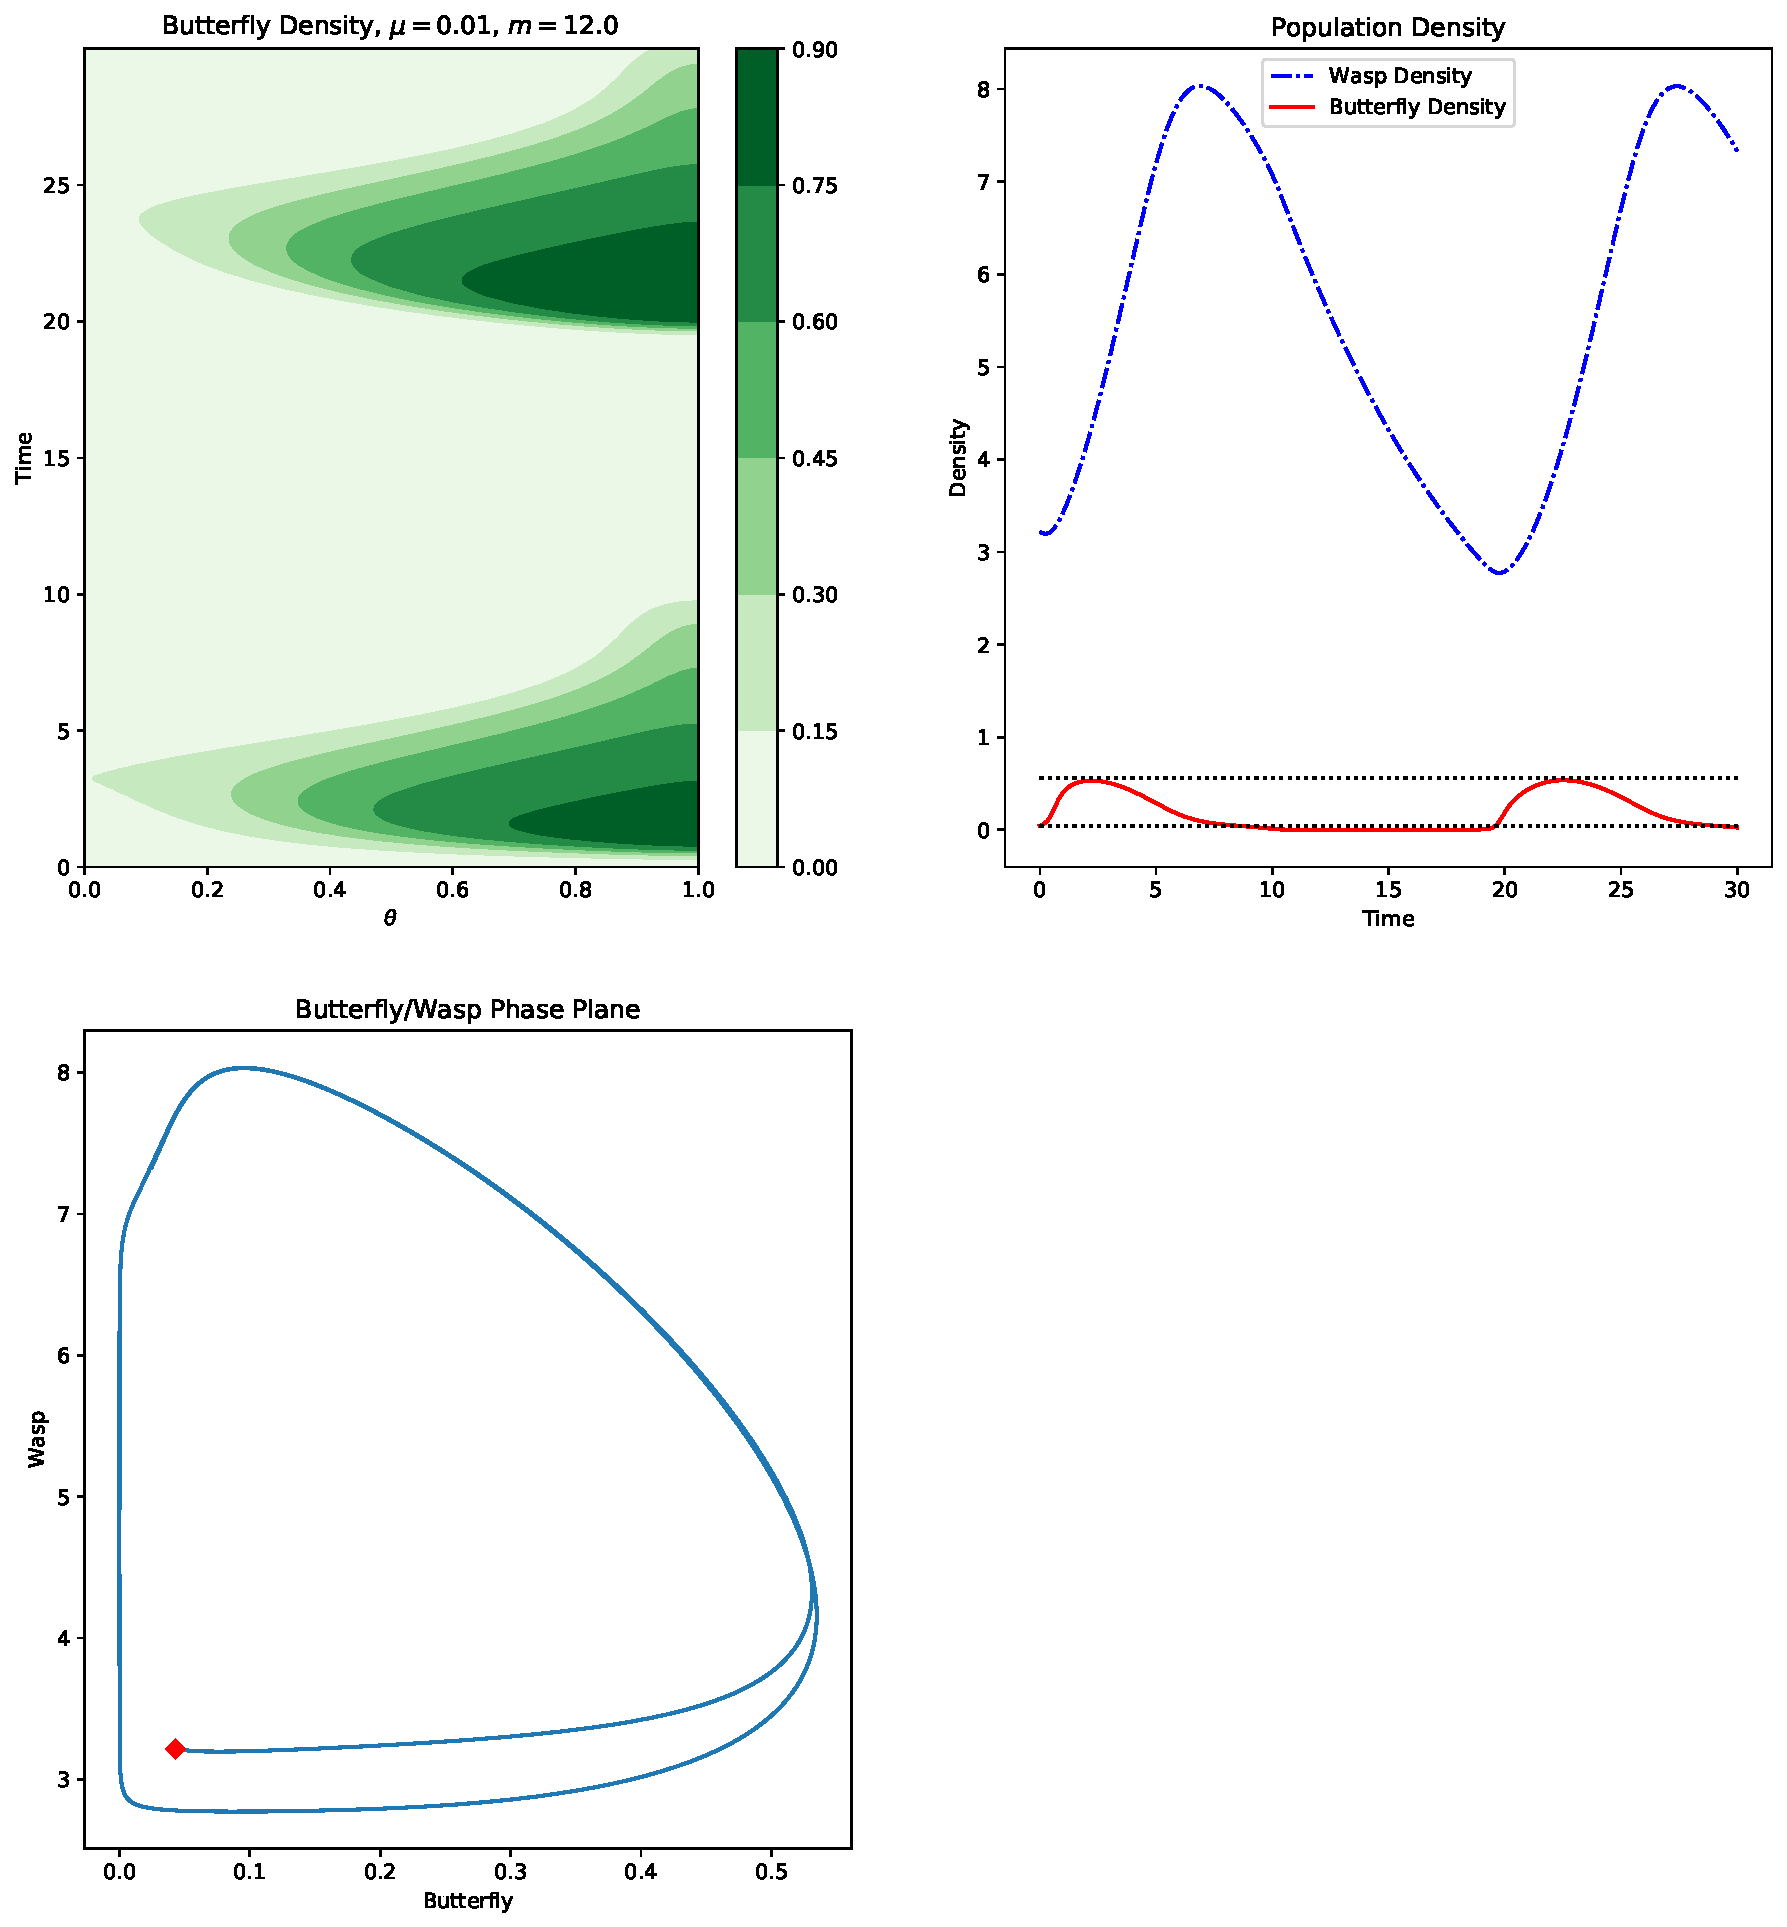
\includegraphics[width=12cm]{img/approximation-mu-01-m-12.pdf}
  \caption[Approximation with $m=12$ and $\mu=0.01$.]{Approximation of
    the system, $m=12$, $\mu=0.01$, $c=2.8$, $g=0.6$, and $d=0.1$. }
  \label{fig:approximationM12Mu01}
\end{figure}

\begin{figure}[htb]
  \centering
  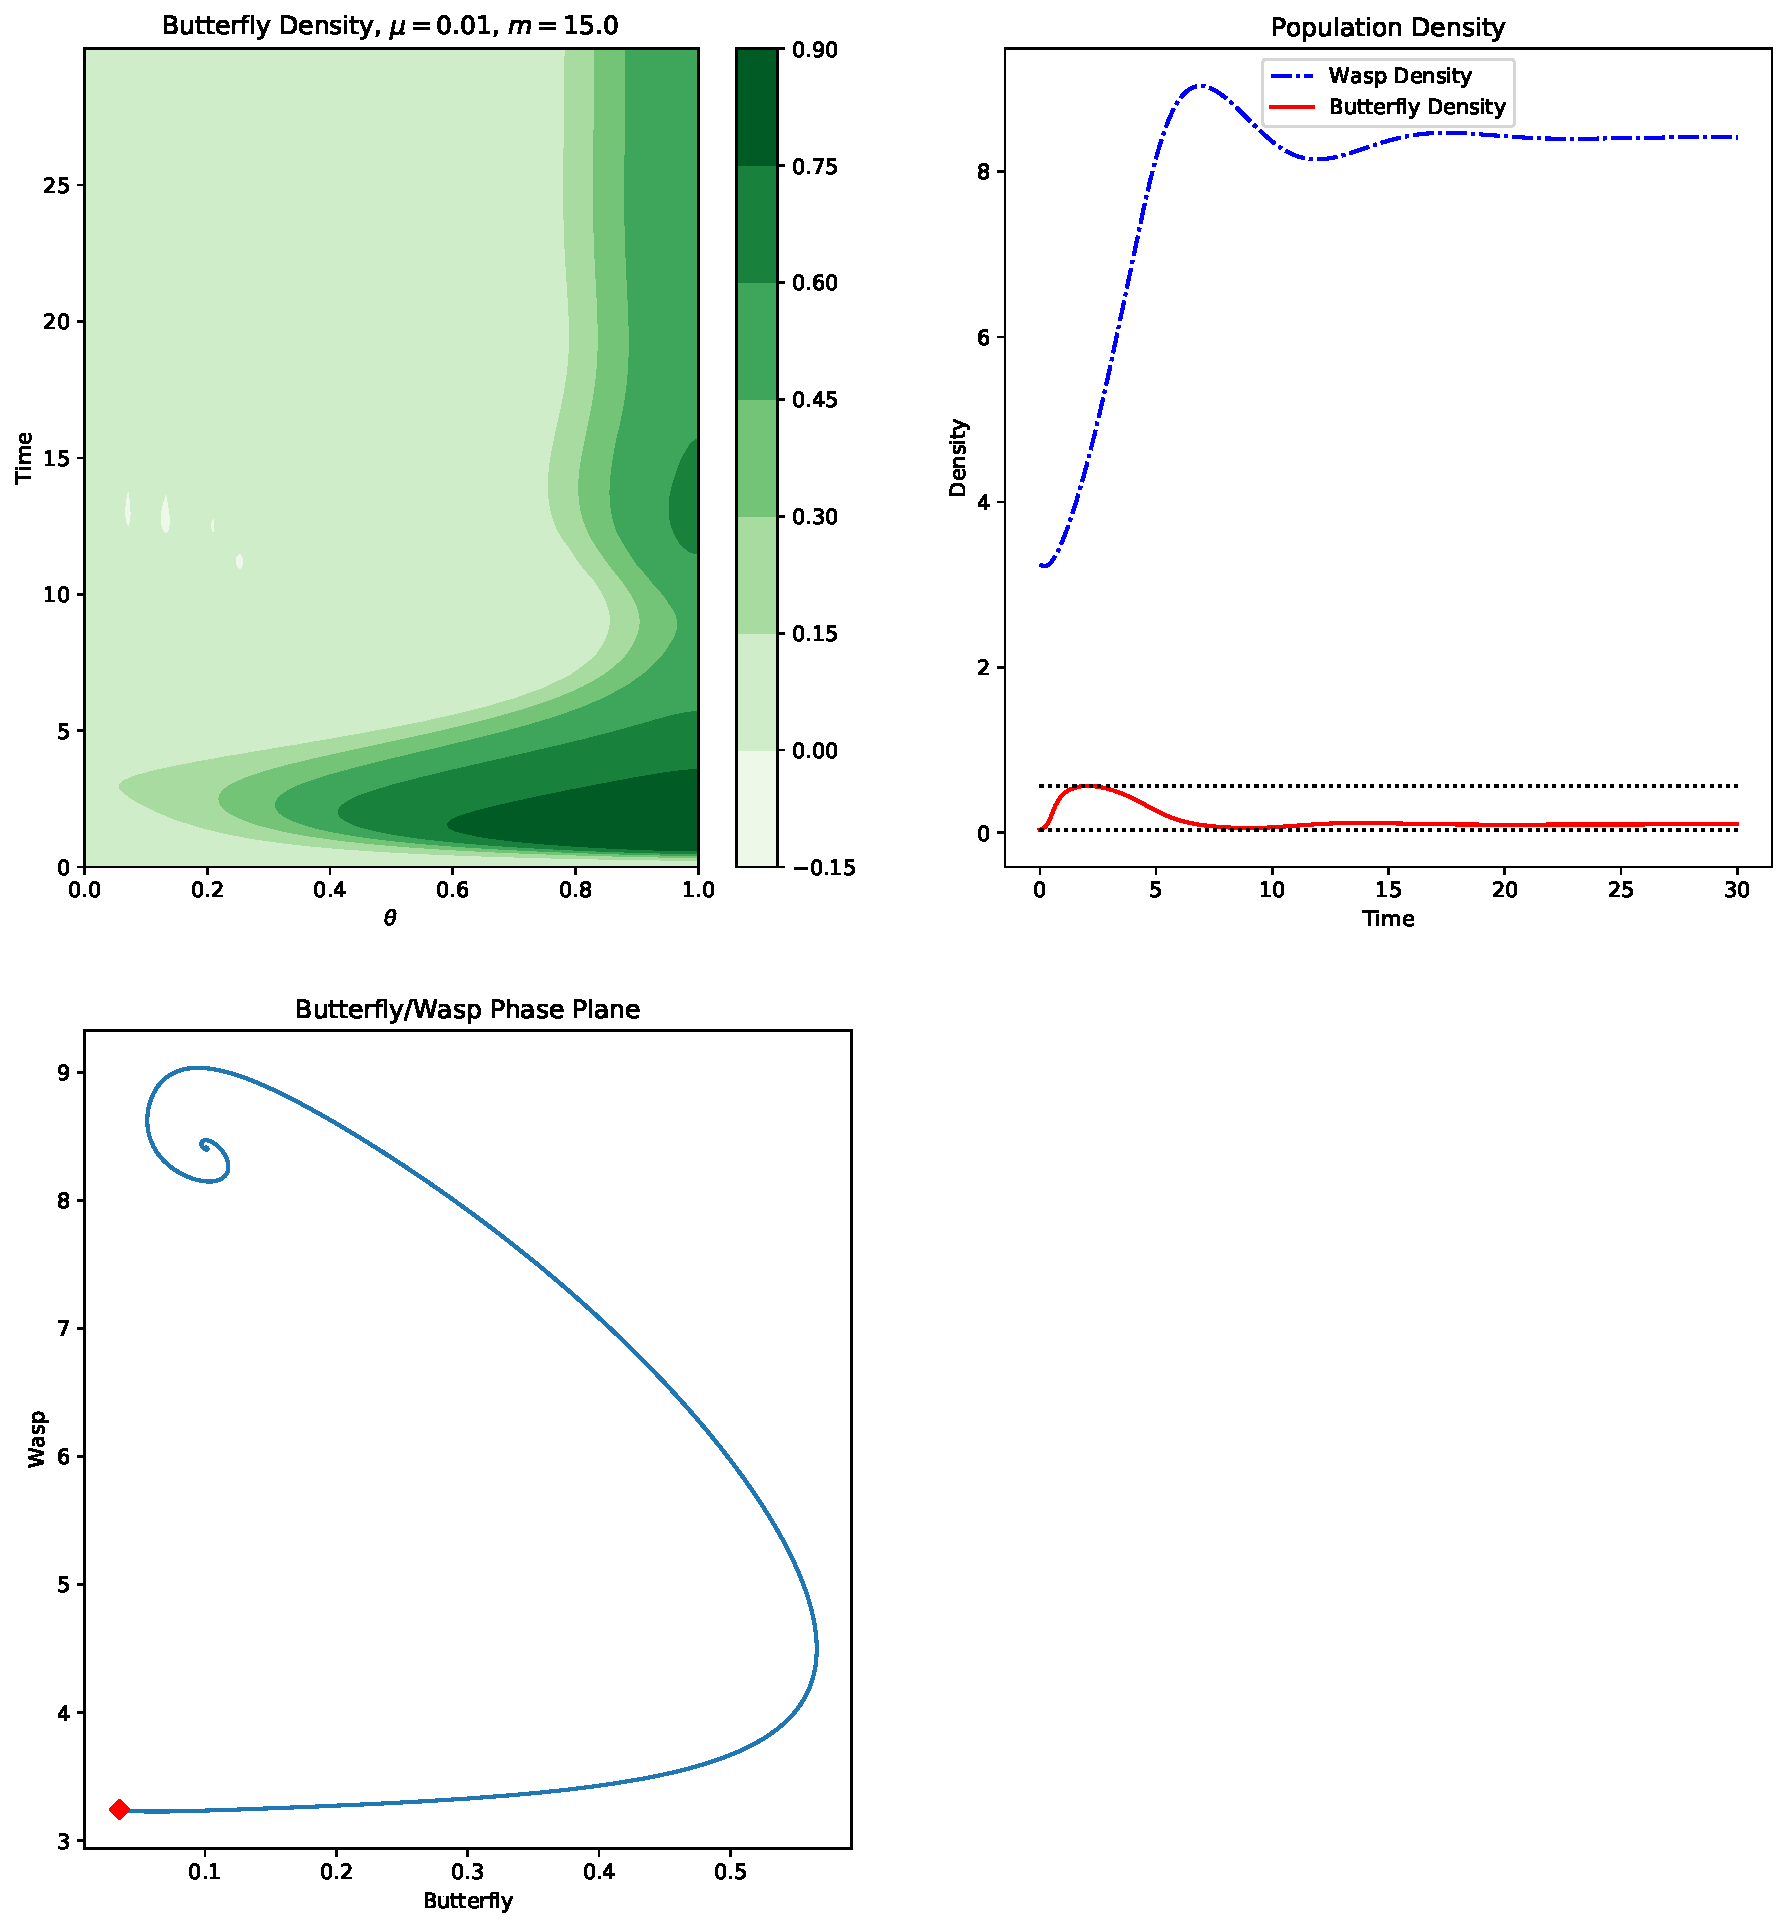
\includegraphics[width=12cm]{img/approximation-mu-01-m-15.pdf}
  \caption[Approximation with $m=15$ and $\mu=0.01$.]{Approximation of
    the system, $m=15$, $\mu=0.01$, $c=2.8$, $g=0.6$, and $d=0.1$. }
  \label{fig:approximationM15Mu01}
\end{figure}

\begin{figure}[htb]
  \centering
  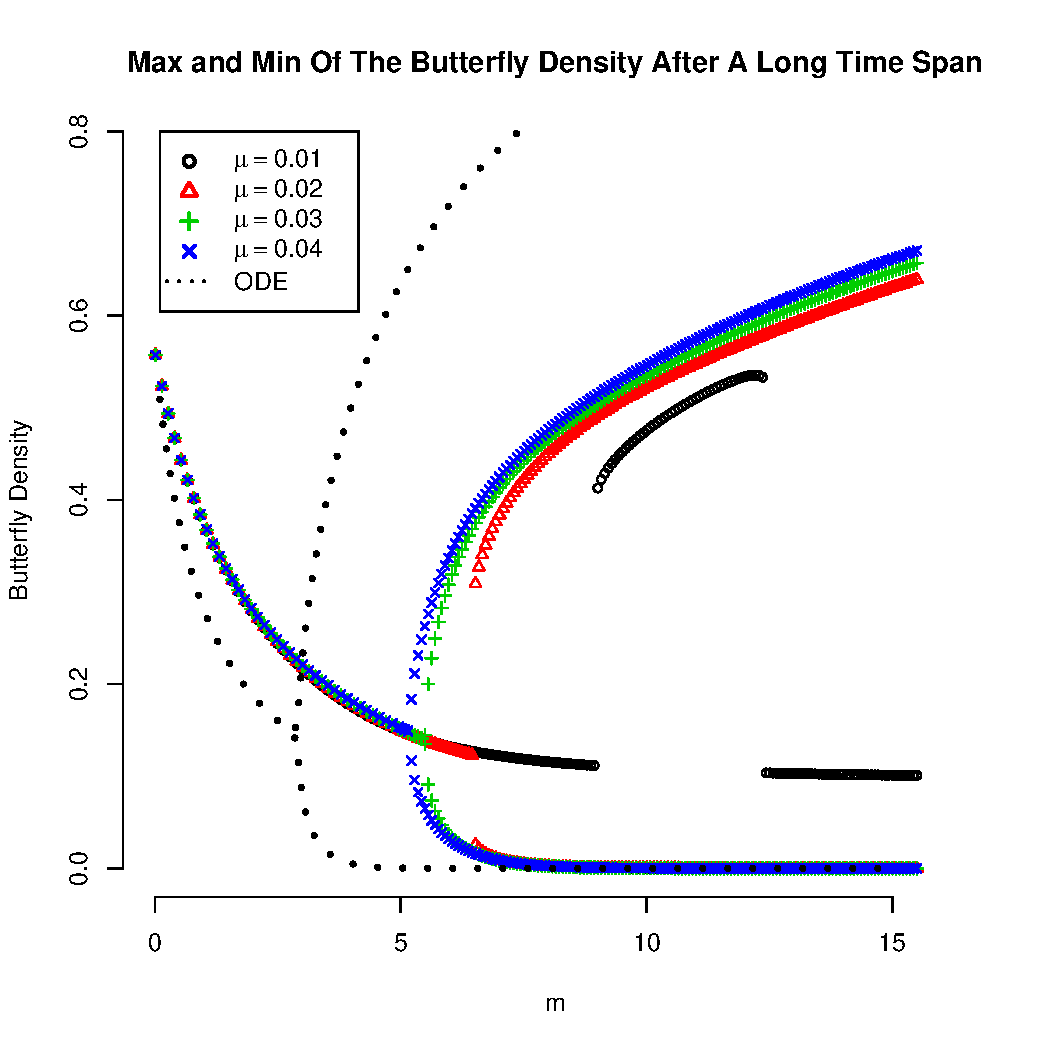
\includegraphics[width=12cm]{img/maxMinByM-mu-01-04.pdf}
  \caption[Maximum and minimum values of the butterfly
  density]{Maximum and minimum values of the butterfly densities after
    a long time period as the parameter $m$ varies.}
  \label{fig:maxMinButterflySmallMu}
\end{figure}

\section{Conclusion}

\section{Acknowledgements}

\clearpage

\appendix

\section{The Fixed Points On The $b$ and $w$ Axes}
\label{appendix:otherFixedPoints}

In subsection \ref{subsection:parameters} the stability of the
non-trivial fixed point is examined. More details about the other
fixed points as well as more complete description of the Jacobian of
the system given in equations (\ref{eq:scaledODE1}) and
(\ref{eq:scaledODE2}) are provided here. In particular the other two
fixed points are given, then the Jacobian is stated, and the linear
stability at the other two fixed points is briefly explored.

The fixed point for the he system of equations given in equations
(\ref{eq:scaledODE1}) and (\ref{eq:scaledODE2}) has one fixed point
where both $b>0$ and $w>0$. There are two other fixed points as
well. One is the fixed point at the origin, $b=0$ and $w=0$.
The remaining fixed point occurs at $w=0$ and $b=\frac{c\cdot
  d}{p(\theta)\left(g - d\right)}$.

The stability at these two fixed points can be examined by first
determining the Jacobian of the system,
\begin{eqnarray*}
  J & = & \left[
          \begin{array}{rr}
            J_{11} & J_{12} \\
            J_{21} & J_{22}
          \end{array}
          \right].
\end{eqnarray*}
The values of the entries in the matrix are
\begin{eqnarray*}
  J_{11} & = & p(\theta)\left(1-2b\right) -
               \frac{w\cdot c \cdot p(\theta)}{\left( c + p(\theta)b \right)^2}, \\
  J_{12} & = & -\frac{p(\theta)b}{c+p(\theta)b}, \\
  J_{21} & = & g\cdot c \cdot  p(\theta) \frac{1}{\left(c+p(\theta)b\right)^2}, \\
  J_{22} & = & -d + g\cdot c \cdot  p(\theta) \frac{1}{c+p(\theta)b}.
\end{eqnarray*}

For the fixed point at the origin, the Jacobian can be expressed as 
\begin{eqnarray*}
  J & = & \left[
          \begin{array}{rr}
            p(\theta) & 0 \\
            0 & -d
          \end{array}
          \right].
\end{eqnarray*}
it is assumed that both $p(\theta)$ and $d$ are non-negative, so the
linear stability at the origin is semi-stable.

For the fixed point at $w=0$ and
$b=\frac{c\cdot d}{p(\theta)\left(g - d\right)}$, the Jacobian can be
expressed as 
\begin{eqnarray*}
  J & = & \left[
          \begin{array}{rr}
            p(\theta)\left( 1 -
            \frac{2c\cdot d}{p(\theta)(g-d)} \right) & -\frac{d}{g} \\
            0 & 0
          \end{array}
          \right].
\end{eqnarray*}
As described in subsection \ref{subsection:parameters} it is assumed
that $g>d$. In order for this fixed point to be stable in the
direction associated with the non-zero eigenvalue then we have that
\begin{eqnarray*}
  p(\theta) & < & \frac{2cd}{g-d}.
\end{eqnarray*}


\section{Stability of the Equilibria}
\label{appendix:stability}

The linear stability with respect to the parameters for the
non-trivial fixed points is examined in subsection subsection
\ref{subsection:parameters}. We now turn out attention to the
existence of limit cycles or oscillatory behaviour of the solutions
near the equilbria. Consider the model system, equations
(\ref{eq:scaledODE1}) and (\ref{eq:scaledODE2}). Can the impact
associated with the use of the anti-pheromone destabilize/stabilize
this equilibrium? If so, under what conditions? This is settled via
the following lemma,
\begin{theorem}
  \bigskip\ All solutions of equations (\ref{eq:scaledODE1}) and
  (\ref{eq:scaledODE2}) with initial values
  $b\left( 0\right) ,w\left( 0\right) >0$ are always non-negative
\end{theorem}


\begin{proof}
  Notice that equations (\ref{eq:scaledODE1}) and
  (\ref{eq:scaledODE2}) have the form
\begin{eqnarray}
  b^{\prime}\left( t \right) & = & b(t)X\left( b,w\right), \\
  w^{\prime}\left( t \right) & = & w(t)Y\left( b,w\right)
\end{eqnarray}


If $\ \left( b\left( t\right) ,w\left( t\right) \right)
$ is a solution of such a system, then using an integrating factor
\begin{eqnarray}
\dfrac{d}{dt}\left( e^{\left( -\int_{0}^{t}X(s)ds\right) }b(t)\right) & = & 0
\end{eqnarray}
Consequently,
\begin{eqnarray}
b(t) & = & e^{\left( -\int_{0}^{t}X(s)ds\right) }b(0), \\
w(t) & = & e^{\left( -\int_{0}^{t}Y(s)ds\right) }w(0).
\end{eqnarray}
So for all $t>0$ and $b\left( 0\right) ,w\left( 0\right) >0$ .
\end{proof}

Having established that the solutions are non-negative our attention
now turns to whether or not the solutions are bounded. We can state
that the solutions are bounded in the first quadrant.

\begin{lemma} \label{mm} All the solutions of equations equations
  (\ref{eq:scaledODE1}) and (\ref{eq:scaledODE2}) which start in
  $R_{+}^{2}$ are uniformly bounded.
\end{lemma}

\begin{proof}
For all $R>0$, consider the triangular regions $T_{R}=\left\{ \left(
b(t),w(t)\right) \in R_{+}^{2}:R=b+\frac{1}{g}w\right\} $

Let's assume that $b(t),w(t)$ are any positive solution of equations
(\ref{eq:scaledODE1}) and (\ref{eq:scaledODE2}). Due to the
non-negativity of the solutions it is immediately implied that
\begin{eqnarray}
  \frac{d}{dt}b(t) & \leq & \hat{p}\left( \theta \right) b(t)\left( 1-b(t)\right) 
\end{eqnarray}
This immediately leads to the bound on $b(t)$,
\begin{eqnarray}
  0\leq b(t)\leq 1
\end{eqnarray}
assuming that the initial condition for $b(t)$ is less than one.  We
claim that $T_{R}$ is forward invariant for all sufficiently large
$R.$We need only show that solutions cannot leave $T_{R}$

We show that
$\frac{d}{dt}\left( b(t)+\frac{1}{g}w(t)\right) =\frac{d}{dt}%
\left( R\right) <0$,
\begin{eqnarray}
  \frac{d}{dt}\left( R\right) & = & \frac{d}{dt}\left( b(t)+\frac{1}{g}w(t)\right), \\
                              & = & \left( \hat{p}\left( \theta \right) b(t)
                                    \left( 1-b(t)\right) -
                                     \frac{d}{g}w\left( t\right) \right), \\
                              & = & \hat{p}\left( \theta \right) b(t)\left(1-b(t)\right) -
                                    d\left( R-b(t)\right), \\
                              & \leq & 0.
\end{eqnarray}


In particular, if $R$ is chosen large enough.
\end{proof}
\begin{theorem}
  \index{3} Consider the model equations (\ref{eq:scaledODE1}) and
  (\ref{eq:scaledODE2}). Assume that the following condition $g>d$
  hold
\end{theorem}

\begin{description}
\item[1]  If $%
\hat{p}(\theta )=c+\dfrac{2cd}{g-d},$ then the non trivial equilibrium $%
E^{\ast }=(b^{\ast },w^{\ast })$ is center.

\item[2] If $0<\hat{p}(\theta )<c+\dfrac{2cd}{g-d}$ then the non trivial
equilibrium $E^{\ast }=(b^{\ast },w^{\ast })$ is locally stable.
\end{description}

\begin{proof}
  The non trivial equilibrium $E^{\ast }=(b^{\ast },w^{\ast })$ of the
  model equations (\ref{eq:scaledODE1}) and (\ref{eq:scaledODE2}) will
  be center if $DetJ>0$ and $TraceJ=0$

since $DetJ>0$ all the time then the it only depend on the value of the $%
TraceJ$
\begin{center}
$TraceJ=J_{11}=00$

iff $\hat{p}(\theta )b^{\ast }\left( -1+\dfrac{\hat{p}(\theta )w^{\ast }}{%
\left( c+\hat{p}(\theta )b^{\ast }\right) ^{2}}\right) =0$

iff $\hat{p}(\theta )w^{\ast }=\left( c+\hat{p}(\theta )b^{\ast }\right)
^{2} $

iff $\hat{p}(\theta )\left( 1-b^{\ast }\right) =\left( c+\hat{p}(\theta
)b^{\ast }\right) $

iff $\hat{p}(\theta )-2\hat{p}(\theta )b^{\ast }=c$

iff $\hat{p}(\theta )-\dfrac{2cd}{g-d}=c$

if $\hat{p}(\theta )=c+\dfrac{2cd}{g-d}$
\end{center}

\end{proof}
\begin{figure}[!htp]
\begin{center}
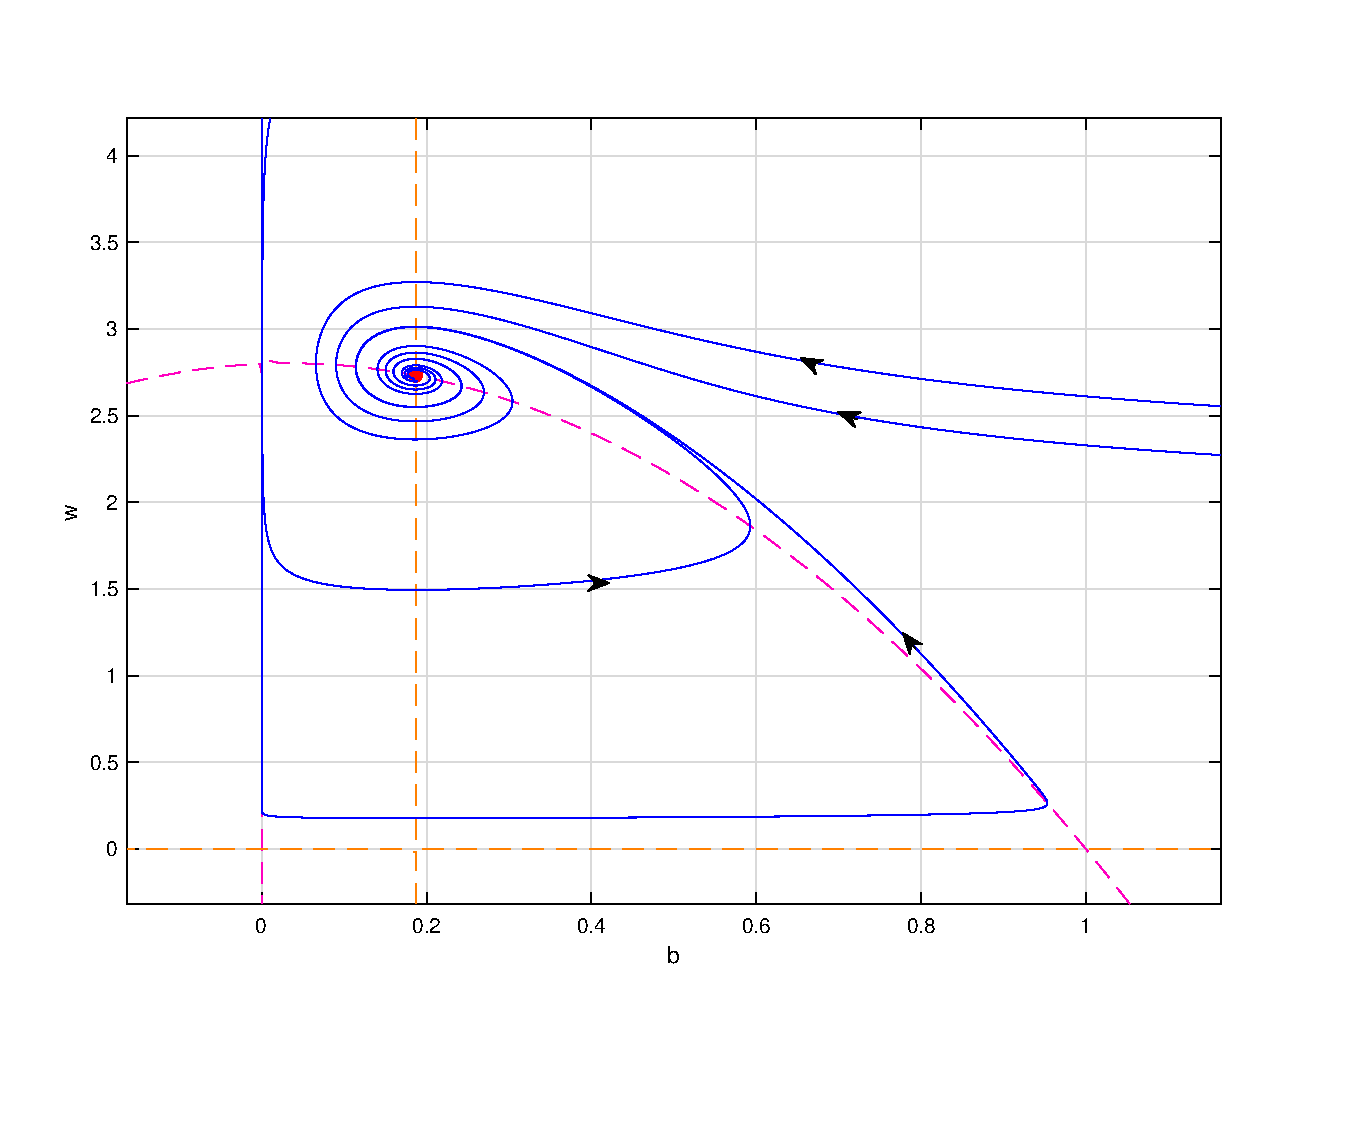
\includegraphics[scale=0.3]{img/s.eps}  

\end{center}

\caption{Figure shows sample runs of $b(t)$ and $w(t)$ for equations
  (\ref{eq:scaledODE1}) and (\ref{eq:scaledODE2}), where
  $\hat{p}(\theta )$ = 3, where the system is stable }
      \label{fig:S}
\end{figure}
%%%%%%%%%%%%%%%%%%%%%%%%%%%%%%%%%%%%%%%%%%%%
\begin{figure}[!htp]
\begin{center}
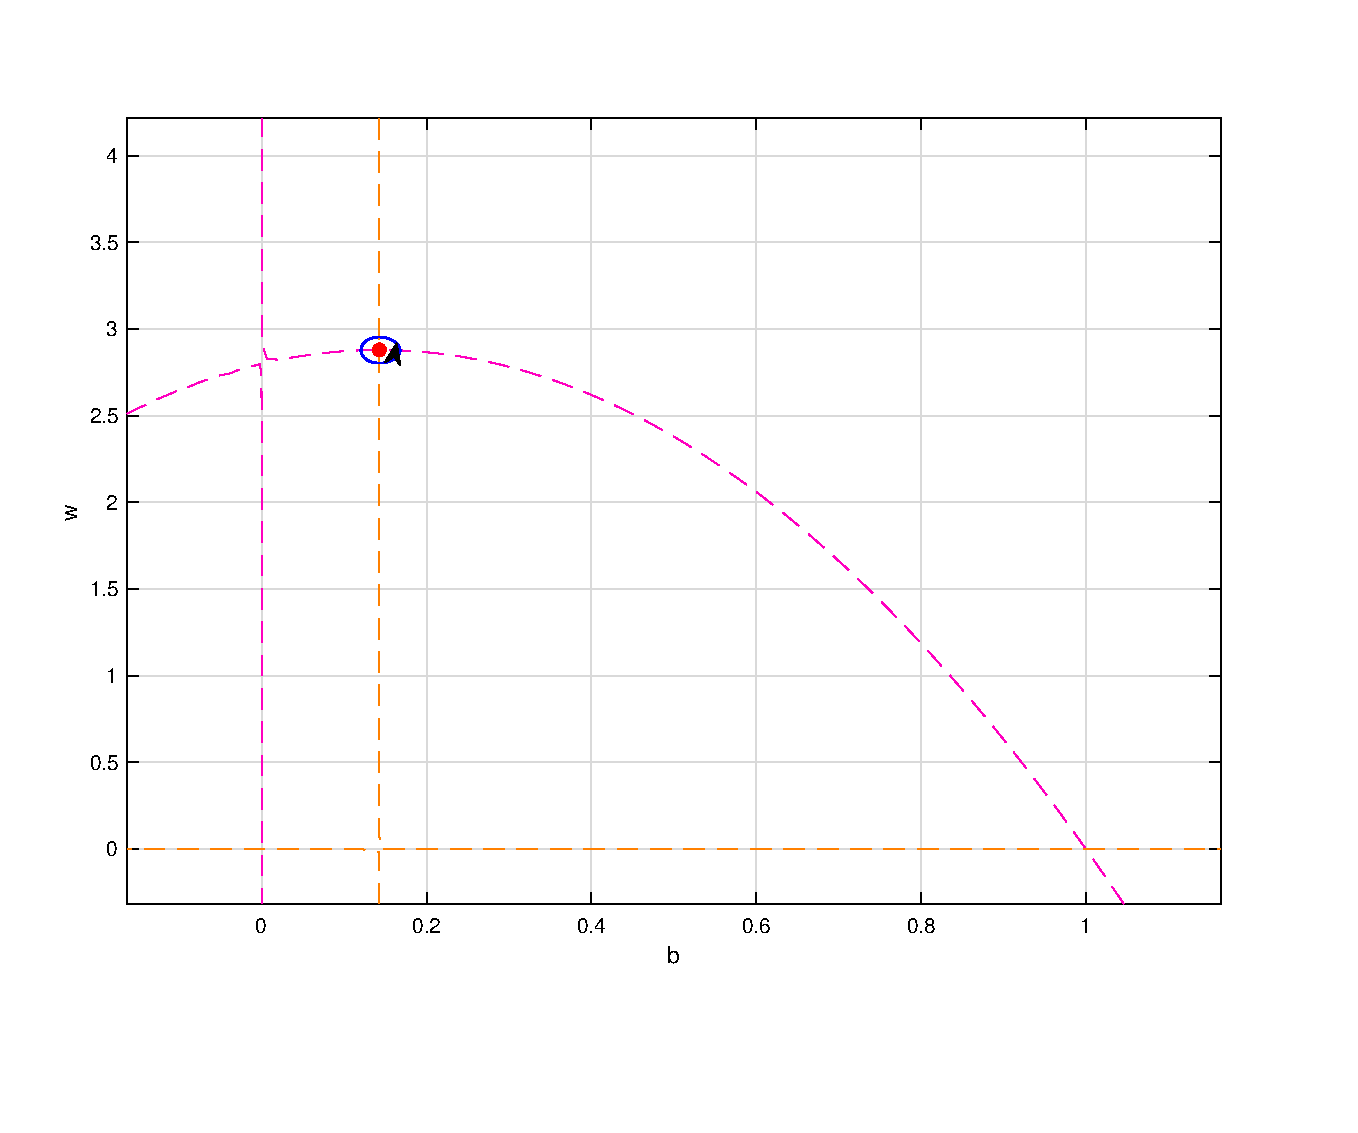
\includegraphics[scale=0.28]{img/l1.eps}  
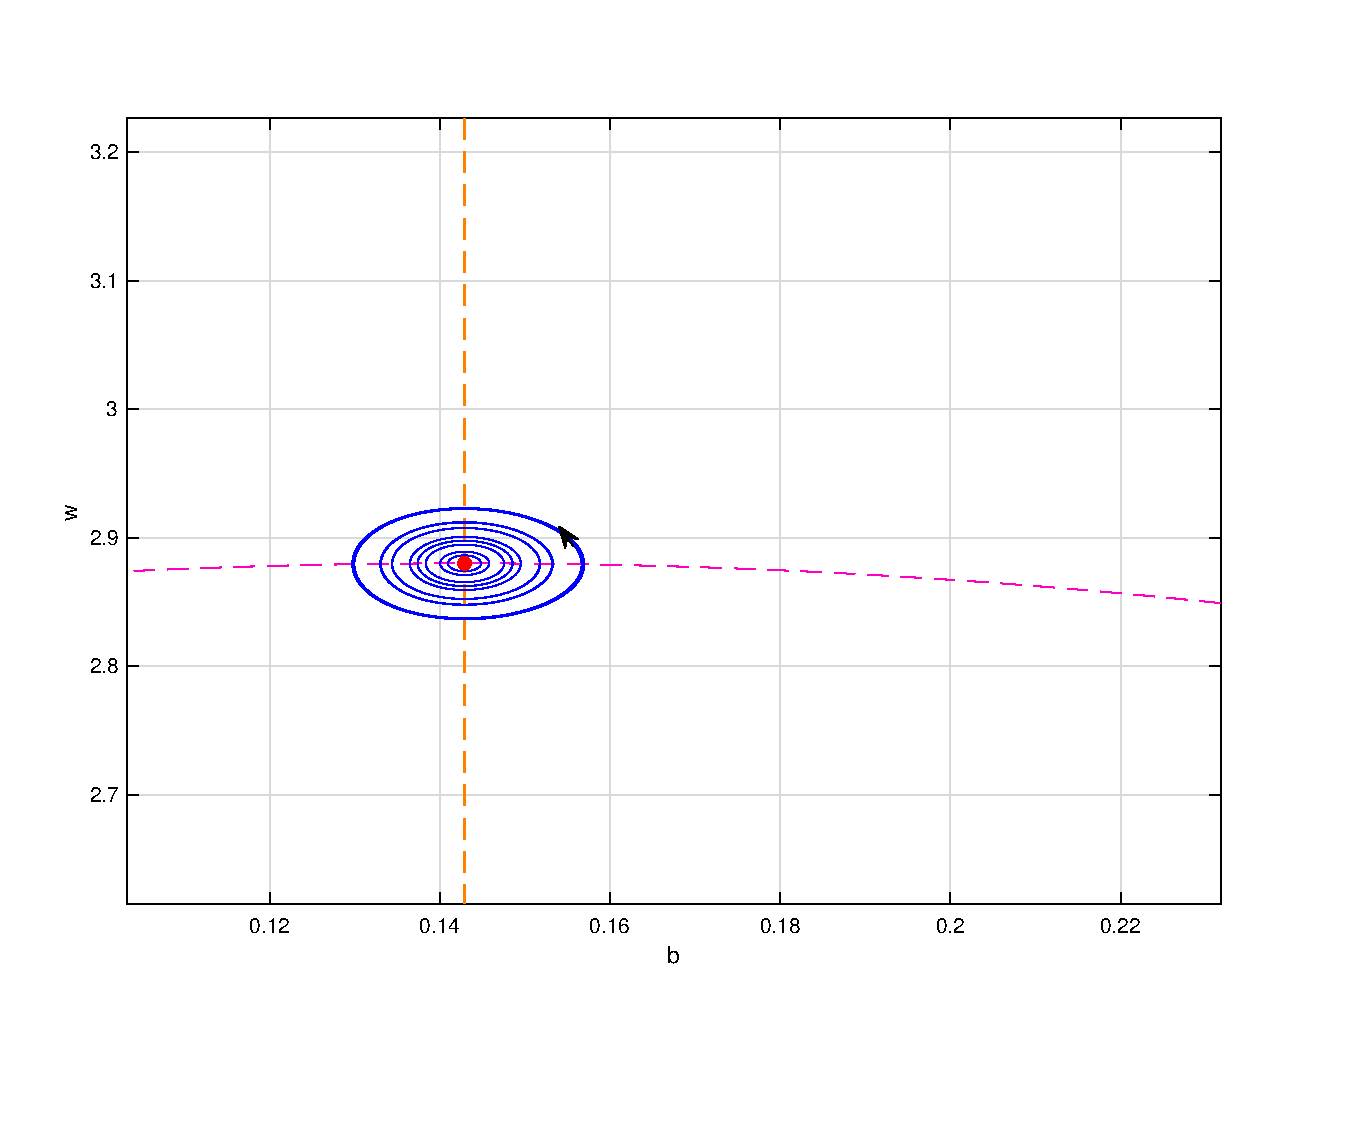
\includegraphics[scale=0.28]{img/l2.eps}

\end{center}

\caption{Figure shows runs of $b(t)$ and $w(t)$ for equations
  (\ref{eq:scaledODE1}) and (\ref{eq:scaledODE2}) has center
  equilibrium point, where $\hat{p}(\theta )=3.92$. }
      \label{fig:l1l2}
\end{figure}

In the next theorem we aim to investigate the effect of the impact
associated with the use of the anti-pheromone $\hat{p}(\theta )$ on
the limit cycle dynamics in equations (\ref{eq:scaledODE1}) and
(\ref{eq:scaledODE2}).

\begin{theorem}
  \index{4} Consider the model equations (\ref{eq:scaledODE1}) and
  (\ref{eq:scaledODE2}). Assume that $E^{\ast }=(b^{\ast },w^{\ast })$
  is the positive non trivial equilibrium point of the model equations
  (\ref{eq:scaledODE1}) and (\ref{eq:scaledODE2}) with \ $g>d$ and the
  following condition hold
\end{theorem}

\begin{center}
$%
\hat{p}(\theta )>c+\dfrac{2cd}{g-d}>0,$
\end{center}

then the system possesses at least one closed loop in the first quadrant.

\begin{proof}
  From the local stability analysis, we have that if the above
  conditions hold, then the positive equilibrium
  $E^{\ast }=(b^{\ast },w^{\ast })$ of equations (\ref{eq:scaledODE1})
  and (\ref{eq:scaledODE2}) is an unstable node or focus. The
  existence of a closed loop now follows from Lemma \ref{mm} and
  Poincair'e--Bendixson theorem \cite{nonlinearChaos}.
\end{proof}

\begin{figure}[!htp]
\begin{center}
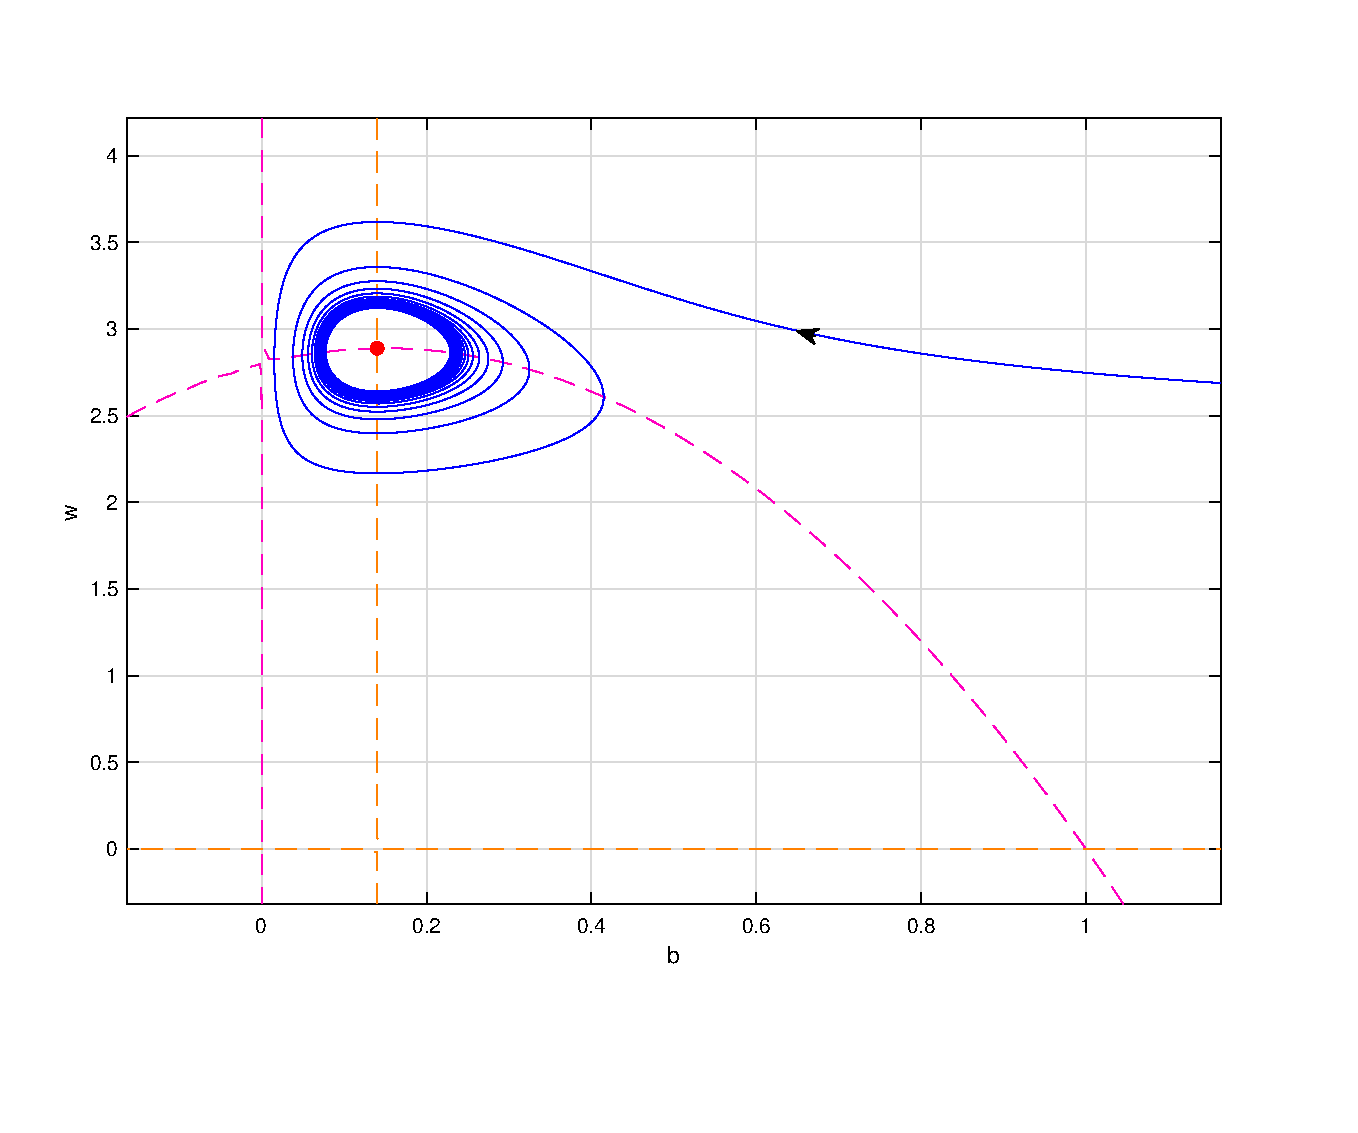
\includegraphics[scale=0.3]{img/lim.eps}  

\end{center}

\caption{Figure shows sample runs of $b(t)$ and $w(t)$ for equations
  (\ref{eq:scaledODE1}) and (\ref{eq:scaledODE2}) , where
  $\hat{p}(\theta )$ = 4, where the system has a limit cycle }
      \label{fig:lim}
\end{figure}


\section{Numerical Approximation}
\label{numericalApproximation}

We introduce the method for the numerical approximation of the coupled
PDE and ODE system in equations (\ref{eq:scaledodePDE1}) and
(\ref{eq:scaledodePDE2}). For the full system, we make use of a
Legendre pseudo-spectral collocation
method\cite{spectralMethodsFluids,hesthaven_gottlieb_gottlieb_2007,gottlieb1977numerical}. First,
the butterfly density is discretized in $\theta$ as
\begin{eqnarray}
  \label{eqn:spatialDiscretization}
  b_N(t,\theta) & = & \sum^N_{i=0} \hat{b}_i(t) \phi_i(\theta),
\end{eqnarray}
where $\phi_i(\theta)$ is the Lagrange interpolant on the
$i$\textsuperscript{th} abscissa of the Legendre-Gauss-Lobatto
quadrature\cite{hesthaven_gottlieb_gottlieb_2007}.

The abscissa of the Legendre-Gauss-Lobatto quadrature are the zeroes
of the function
\begin{eqnarray}
  \psi(\theta) & = & \left(1-\theta^2\right) L_{N}'(\theta),
\end{eqnarray}
where $L_N(\theta)$ is the $n$\textsuperscript{th} Legendre
polynomial\cite{davis2007methods}.  The weights, $w_n$, associated
with the quadrature are identical to those described in
Davis\cite{davis2007methods} as well as Golub and
Welsch\cite{gaussQuadratureRules}. In our examples the quadrature is
approximated using the methods described by Golub and
Welsch\cite{gaussQuadratureRules}.  Given $\psi(\theta)$ the Lagrange
interpolants can be calculated
\begin{eqnarray}
  \phi_i(\theta) & = & \frac{\psi(\theta)}{\psi'(\theta)(\theta-\theta_i)}.
\end{eqnarray}
The function $\psi(\theta)$ coincides with the Legendre differential
equation, and the relationship can be simplified as
\begin{eqnarray}
  \psi'(\theta) & = & -N(N+1)L_N(\theta).
\end{eqnarray}

The discretization of equations (\ref{eq:scaledodePDE1}) and
(\ref{eq:scaledodePDE2}) is constructed by substituting the definition
of $b_N$ from equation (\ref{eqn:spatialDiscretization}). A Galerkin
approximation is constructed, and one minor complication is that the
Lagrange interpolants are polynomials of degree $N$, and the
Gauss-Lobatto quadrature is exact for polynomials up to degree
$N$. The integral is approximated using the Gauss-Lobatto quadrature,
and the resulting sum results in an equivalent norm compared to the
Gauss quadrature which is exact for polynomials up to degree
$N$\cite{SobolevCanutoQuarteroni}.

The resulting variational form for Neumann boundary conditions using a
Galerkin approximation and a discrete inner product for equation
(\ref{eq:scaledodePDE1}) is
\begin{eqnarray}
  \sum_{j=0}^N \sum_{i=0}^N  \hat{b}_i'(t) \phi_i(\theta_j) \phi_k(\theta_j) w_j
  & = &
  \sum_{j=0}^N \sum_{i=0}^N \hat{p}(\theta_j)  \hat{b}_i(t) (1 - \hat{b}_i(t) ) \phi_i(\theta_j) \phi_k(\theta_j) w_j \\
  & &  -  \sum_{j=0}^N w(t) \frac{\hat{p}(\theta_j) \sum_{i=0}^N \hat{b}_i(t) \phi_i(\theta_j) }{c+\hat{p}(\theta_j) \sum_{i=0}^N \hat{b}_i(t) \phi_i(\theta_j)} \phi_k(\theta_j) w_j \nonumber \\ 
  & & - \sum_{j=0}^N \mu  \sum_{i=0}^N \hat{b}_i(t) \phi_i'(\theta_j) \phi_k'(\theta_j)  w_j, \nonumber
\end{eqnarray}
for all integer values of $k$ from $0$ to $N$ inclusive.  The basis
functions are the Lagrange interpolants on the abscissa, and the
equations can be reduced to
\begin{eqnarray}
  \hat{b}_k'(t) 
  & = &
        \hat{p}(\theta_j) \hat{b}_k(t) (1 - \hat{b}_k(t) )
        -  w(t) \frac{\hat{p}(\theta_k) \hat{b}_k(t)) }{c+\hat{p}(\theta_k)  \hat{b}_k(t) }  
   - \frac{\mu}{w_k} \sum_{i=0}^N \hat{b}_i(t) \left( \sum_{j=0}^N  \phi_i'(\theta_j) \phi_k'(\theta_j)  w_j \right).
\end{eqnarray}

Combined with equation (\ref{eq:scaledodePDE2}) the approximation
consists of a system of $N+2$ ordinary differential equations. The
integral in equation (\ref{eq:scaledodePDE2}) is approximated using
the Legendre-Gauss-Lobatto quadrature. The temporal discretization of
the resulting system is constructed using a second order, implicit
multi-step scheme. The scheme is implemented as a fully implicit
second order Adams-Moulton scheme\cite{ascher2011first}. At each time
step the resulting non-linear system is approximated using Newton's
method.


\clearpage
\bibliographystyle{siam}
\bibliography{animalBehaviour}


\end{document}
